% ============================================== %
% INTRODUCTION %
% ============================================== %

\section{Introduction}

% Prolog / Background %

In the recent years, data visualization tools have become an integral part of data exploration systems. The users who are interested in finding some meaningful insights in data have neither time nor patience to manually generate all possible data visualizations. In addition to time, the domain knowledge is another key factor when generating visualizations manually. However, with an exponential growth of available data in various domains, there has been an increase in the number of \textit{Data Enthusiasts}, people with little domain knowledge and technical expertise, looking for interesting trends in data.

\begin{figure}
	\centering
	\begin{subfigure}[b]{0.40\textwidth}
		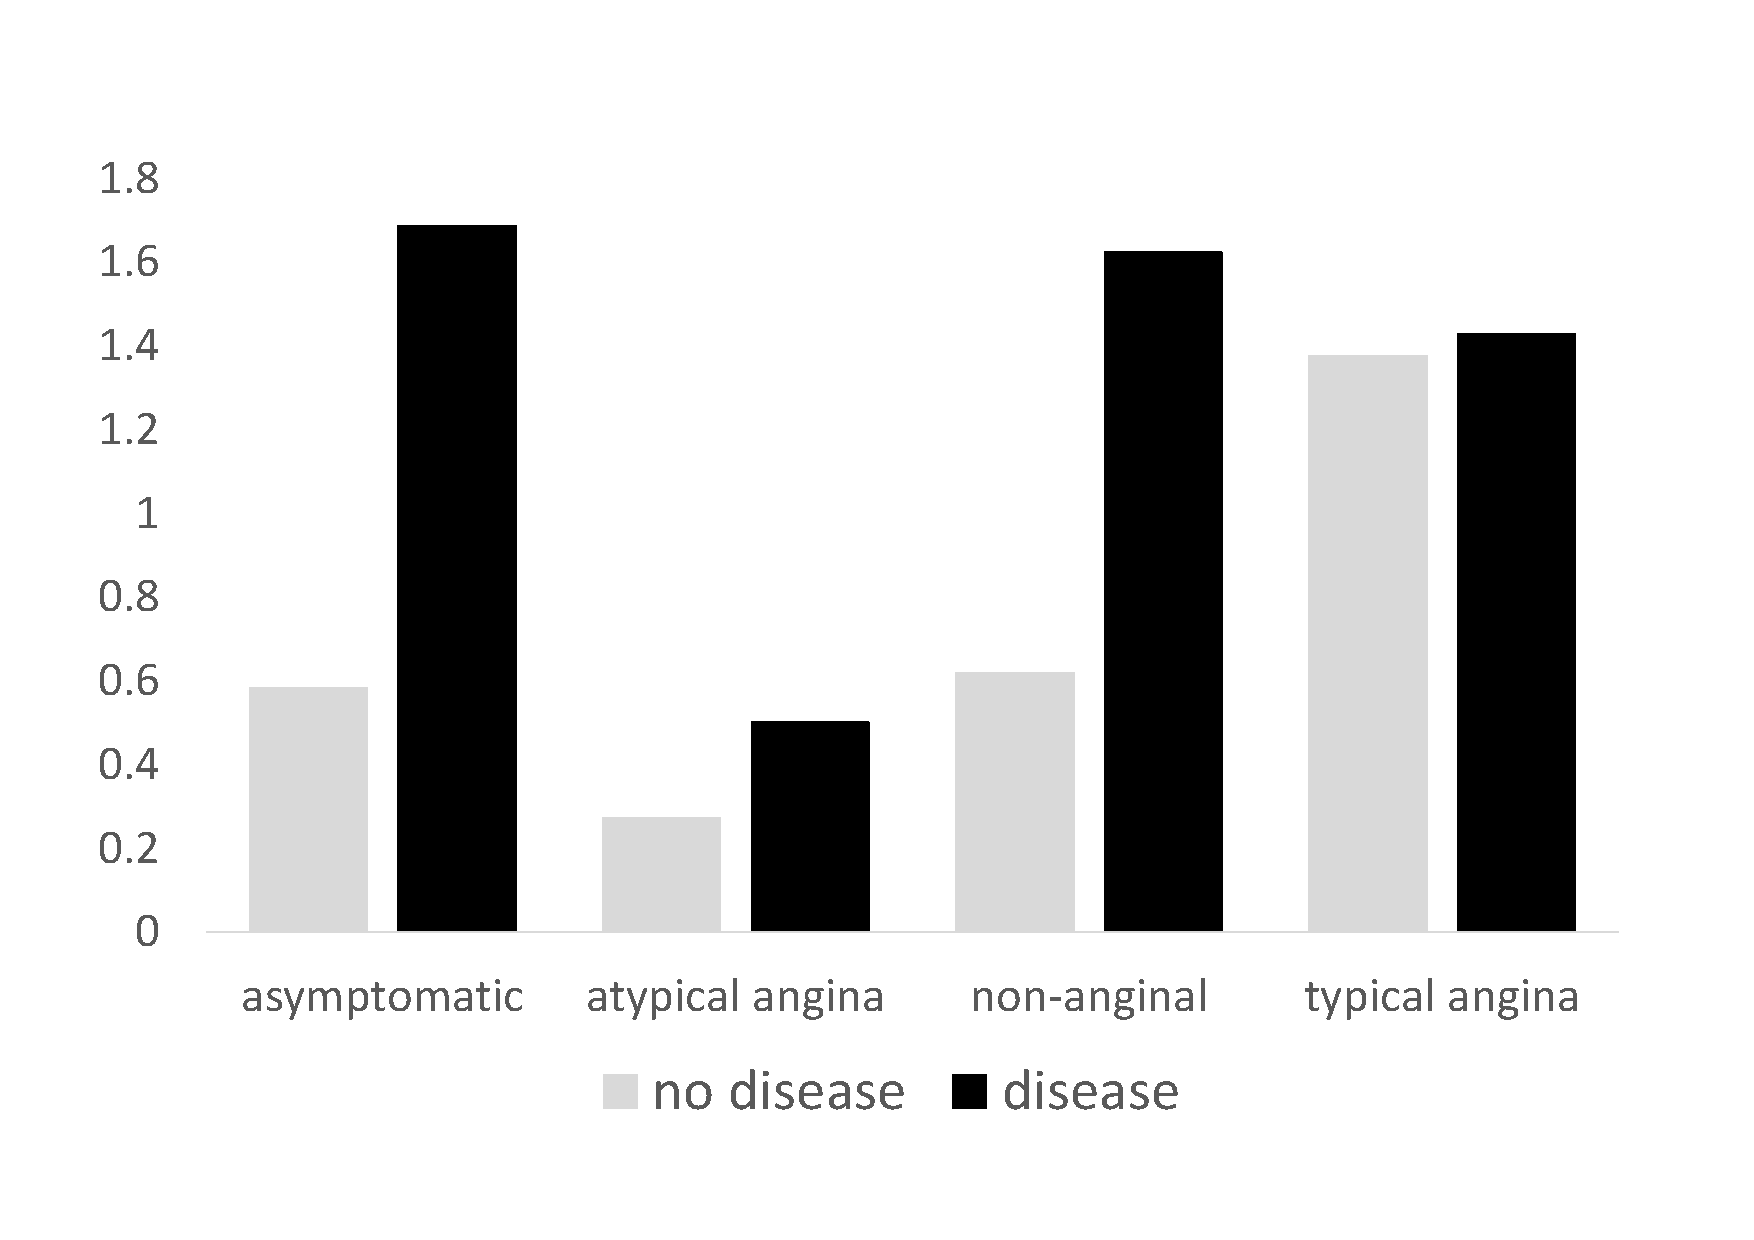
\includegraphics[width=2.5in]{figures/introduction/cp_avg_oldpeak}
		\caption{Visualization of the avg. oldpeak vs. chest pain types}
		\label{fig:intro1} 
	\end{subfigure}
	
	\begin{subfigure}[b]{0.40\textwidth}
		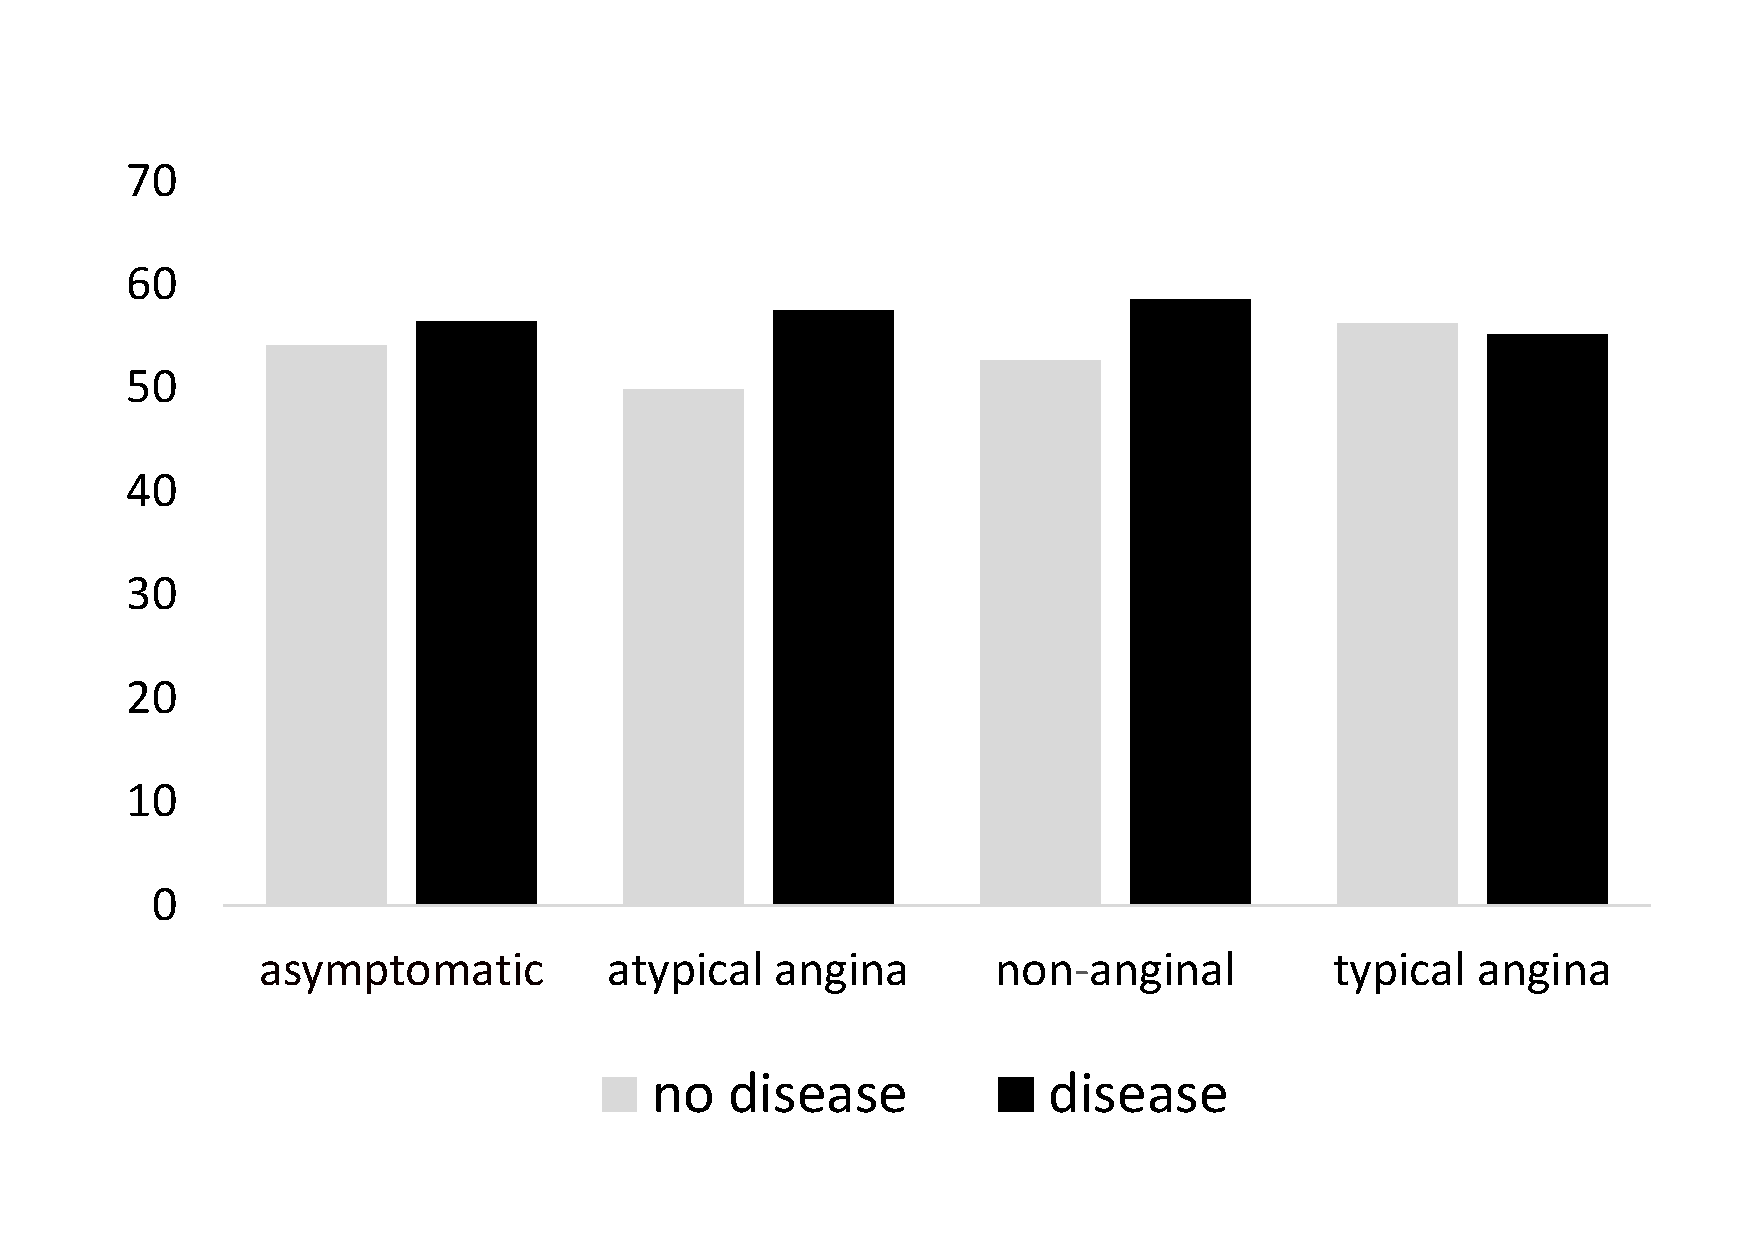
\includegraphics[width=2.5in]{figures/introduction/age_oldpeak}
		\caption{Visualization of the average age vs. chest pain types }
		\label{fig:intro2}
	\end{subfigure}
	\caption[important vs not]{Important vs. less important view.}
\end{figure}

% Example /Case %

For instance, consider a Cleveland heart disease dataset \footnote{http://archive.ics.uci.edu/ml/datasets/heart+Disease}, which describes patients with and without a heart disease.  A data enthusiast might be interested in conducting some comparison between people with heart disease (disease) and people without heart disease (no disease). Without any prior insights about data, she must manually specify different combinations of attributes, measures and aggregate functions before finally generating a visualization that reveals some interesting information about the dataset.  The user effort and time spent in that process increases exponentially with increase in the number of attributes and measures. Hence, several data-driven visualization recommendation tools have been proposed to reduce the user effort and time during data exploration \cite{Vartak2014, Vartak2015, Ehsan2016}. The main goal of those recommendation systems is to provide the user with the most important visualizations (top-k views), which are selected from all possible visualizations. The top-k views are selected based on the most important views in the dataset. The importance of a view is defined on the basis of particular criteria. One of the widely used criteria for importance is based on the deviation between the queried subset of data (target view) with the reference subset of data (reference view). The reference subset can be another subset of the dataset, the rest of the dataset, or the whole dataset. The intuition behind deviation based approach is that views that reveal substantially different trends from the reference views are likely to be of higher interest to the user\cite{Vartak2014, Vartak2015}.  

% Explanation of the example %

Consider again the example of the heart disease dataset. Let the target subset be the data of people with heart disease and the reference subset be the data of people without heart disease. As shown in Figure \ref{fig:intro1} the average oldpeak (pressure of the ST segment) vs. chest pain types is more important view rather than the Figure \ref{fig:intro2} the average of age vs. chest pain types, due to the large deviation between target view (disease) and reference view (no disease) data. Figure \ref{fig:intro1} shows people with heart disease, especially who the chest pain types is asymptomatic tend to have much higher oldpeak rather than people without disease. To the contrary, the Figure \ref{fig:intro2} is potentially less important visualization compared to Figure \ref{fig:intro1}, even there is a deviation between disease and no disease but the deviation is very small and if it is compared to Figure \ref{fig:intro1}, it has lower deviation than Figure \ref{fig:intro1}. Figure \ref{fig:intro2} shows that there is no significant different in term of the average age of the people with four types of chest pain.
\begin{figure}
	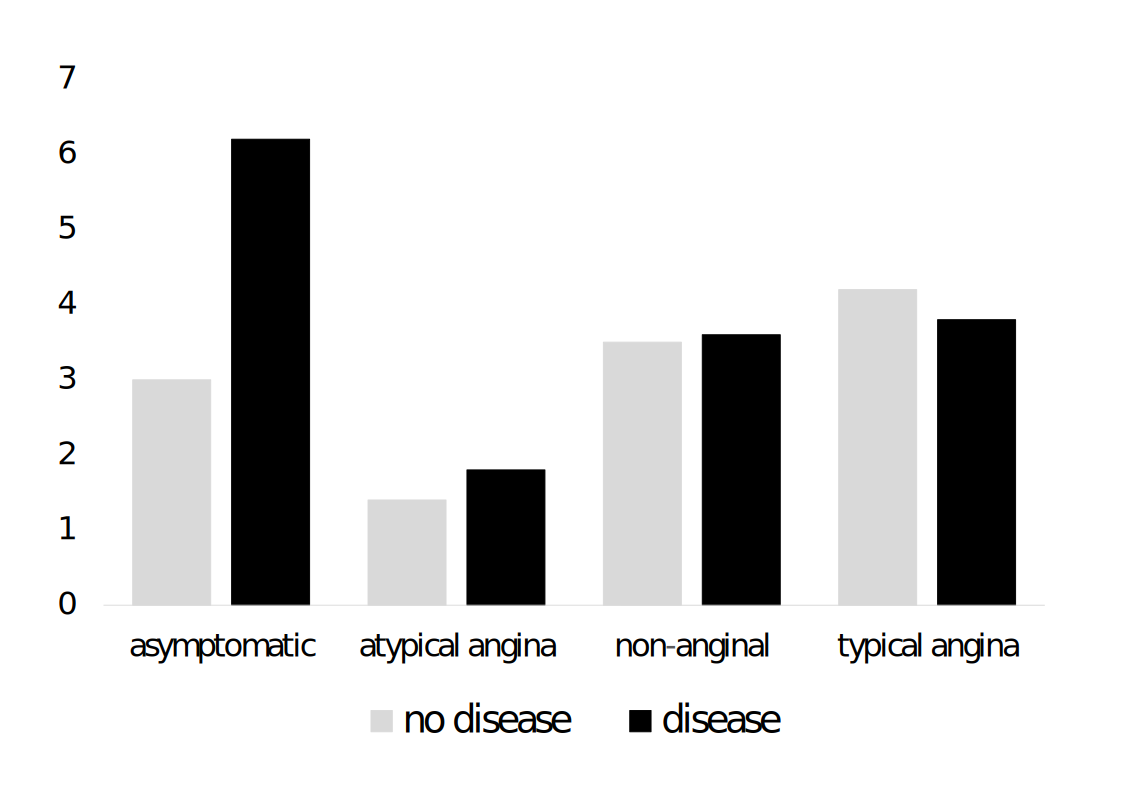
\includegraphics[width=2.5in]{figures/introduction/cp_max_oldpeak}
	\caption{The visualization of maximum oldpeak vs. chest pain types}
	\label{fig:intro3}
\end{figure}

% Problem/Issue in the current solution %

Although the deviation based visualization recommendation systems automatically provide users with the most important visualizations, it is likely that the views in the top-k set might be providing redundant information. For instance, Figure \ref{fig:intro3} provides the information which close to Figure \ref{fig:intro1} that the people with heart disease tend to have higher oldpeak values. Figure \ref{fig:intro3} has same attribute and attribute measure to Figure \ref{fig:intro1}, the only difference is the aggregate function, where Figure \ref{fig:intro1} uses AVG and Figure \ref{fig:intro3} uses MAX. Since both views have a high deviation from the reference subset, both will appear in the top-k set. This leads to an important observation that using only importance as the selection criteria may deliver redundant recommended views, which leads to presents not optimal insights. 

% Proposing Solution %
However, novelty and diversity are one of the fundamental characteristics of any effective recommendation systems \cite{Zhang2008,Clarke2008,Rafiei2010, Yu2009}. Specifically, it is highly desirable that a visualization recommendation systems provides users with views that are both importance and also provide novel information that has not been revealed by the other views. 

% Lists of contributions %
Towards designing an effective visualization recommendation systems that promotes both importance and novelty in recommended views, in this work, we propose an integrated approach called \textit{i-DiVE}. In particular, \textit{i-DiVE} aims to generate top-k visualizations that balance the tradeoff between importance and diversity. The main contributions of this paper are summarized as follows:

\begin{itemize}
	\item We formulate the problem of evaluating recommended views that are both importance and diverse. 
	\item We define a similarity measure to capture the distance between two visualizations.
	\item We present a hybrid objective function to balance the tradeoff between importance and diversity when ranking the visualizations.
	\item We propose the novel \textit{i-DiVE} scheme, that employs various algorithms to evaluate the recommended visualizations based on the hybrid ranking/objective function.
	\item We present optimization techniques that leverage the hybrid objective function to substantially reduce the computational costs.
	\item We conduct an extensive experimental evaluation on real datasets, which compare the performance of various algorithms and illustrate the benefits achieved by \textit{i-DiVE} both in terms of effectiveness and efficiency. 
\end{itemize}


The rest of the paper is organized as follows: in Section II, we formulate the top-k diverse visualization problems and our related work; we present our proposed scheme \textit{i-DiVE}  in Section III; the experimental evaluation is reported in in Section IV and we conclude in Section V.








% ============================================== %
% PRELIMINARIES %
% ============================================== %

\section{PRELIMINARIES AND RELATED WORK}
\subsection{Visualization Recommendation Systems}

% Visualization Recommendation System explanation %

In this work, we consider a visual data exploration session that begins by an analyst submitting a query $Q$ on a multi-dimensional database $D_B$ to be visually analyzed. We assume that the analyst desires to select a subset of $D_B$  by specifying a query predicate $T$. Hence, a general format for query $Q$ can be defined as: 

\bigskip
$Q$ = SELECT * FROM $D_B$ WHERE $T$;
\bigskip

The result of $Q$ is $D_Q$ which is a subset of $D_B$ that need to be visualized.

In order to generate visualizations for $D_Q$, the $D_B$ consists of a set of dimensional attributes $\mathbb{A}$ and a set of measure attributes $\mathbb{M}$. Also, let $\mathbb{F}$ be a set of possible aggregate functions over measure attributes, such as COUNT, AVG, SUM, MIN and MAX. Using different combinations of dimension and measure attributes along with various aggregate functions, and specifying GROUP BY, it is possible to execute aggregate queries over $D_Q$.  %Each aggregate query generates a two column result, where column one consists of attribute dimension values and second column presents the corresponding aggregate function values on measure attribute.
The result generated by the aggregate query can be easily visualized as bar charts. 

For instance, consider again example 1. Let $D_B$ be Cleveland heart disease data table (e.g., tb\_heart\_disease). The analyst wants to do comparison between people with heart disease (disease) and people without heart disease (no disease). This example leads us to the two subsets which are disease subset as the target subset $D_T$ and no disease subset as the reference subset $D_R$.
Hence, each of the subset, leads to a unique visualization called a target view denoted as $V_T$ and a reference view denoted as $V_R$. We can formally define as: 

\bigskip
$V_T$  = SELECT $A$, $F$ ($M$) FROM $D_B$ WHERE $T_T$ GROUP BY $A$;

$V_R$  = SELECT $A$, $F$ ($M$) FROM $D_B$ WHERE $T_R$ GROUP BY $A$;
\bigskip

where $A \in \mathbb{A}$, $M\in \mathbb{M}$, and  $F \in \mathbb{F}$. We consider the attribute and measure dimensions of $D_B$ which are; $\mathbb{A}$ =  (chest\_pain\_types), $\mathbb{M}$ = (age, oldpeak) and $\mathbb{F}$ = (COUNT, AVG, SUM, MIN and MAX). The query predicate $T_T$ is \quotes{status = Disease}, this predicate generates a subset $D_T$ of $D_B$ that contains data of all patients with heart disease. Meanwhile, the query predicate $T_R$ is \quotes{status = No Disease} which generate subset $D_R$ of $D_B$ and it consists the data of all patients without heart disease. Using various combinations of attributes, measures and aggregate functions, it is possible to generate 2 * | $\mathbb{A}$ |*| $\mathbb{M}$ |*| $\mathbb{F}$ | = 2*(1*2*5) = 20 views. For instance, the views shown in Figure \ref{fig:intro1} and \ref{fig:intro2} correspond to $A$=\quotes{chest\_pain\_types}, $M$=\quotes{age}, \quotes{oldpeak}, and $F$=\quotes{Avg}. In addition, the view of Figure \ref{fig:intro3}  corresponds to $A$=\quotes{chest\_pain\_types}, $M$=\quotes{oldpeak}, and $F$=\quotes{Max}.

It is clear from the above example that even for a modest dataset that only has one attribute and two meassure attributes, the number of possible views to consider can be large. Also, not all the views will be of interest to the user. Therefore, in order to reduce the user effort, it is very important to recommend a set of few \quotes{most important} views. The challenge, however, is to determine what constitutes the most imporant of set of views. Most of the existing visualization recommendation systems techniques rely mainly on the content of the view in terms of data generated as a result of the underlying aggregate query\cite{Vartak2015}, \cite{Vartak2014}. Those exiting approaches lead to recommend homogeneous views as explained in the introduction section.%The recommendation approach results in a set of views that are individually interesting in reference to some other subset of data or the whole data set. Since the views are recommended as a collection or set of multiple views, the quality of the whole set is as important as the quality of individual views\cite{Vartak2017}. 

Therefore, in this work, we consider the content of a view as well as its context. The content of a view is determined by the data presented in the view and the context of the view is determined from the attributes, meassures and aggregate functions of the query. 
%\bigskip
%$V_{Tcontent}$ = SELECT $A, F$($M$) FROM $D_Q$ GROUP BY $A$;
%
%$V_{Tcontext}$= [$A, F, M$]
%\bigskip

\subsection{Content and Context Driven}
In the process to recommend users a set of important views, we work at two levels. At the first level, we evaluate that how \quotes{important} is the content of the view as compared to other subsets of data. In particular, we determine how different are the trends and patterns revealed by $V_{T}$ from some reference data subset $V_{R}$ in terms of content. At the second level, we evaluate contextually how different a view is from other views in the recommended set. 

\begin{figure}
	\centering
	\begin{subfigure}[b]{0.40\textwidth}
		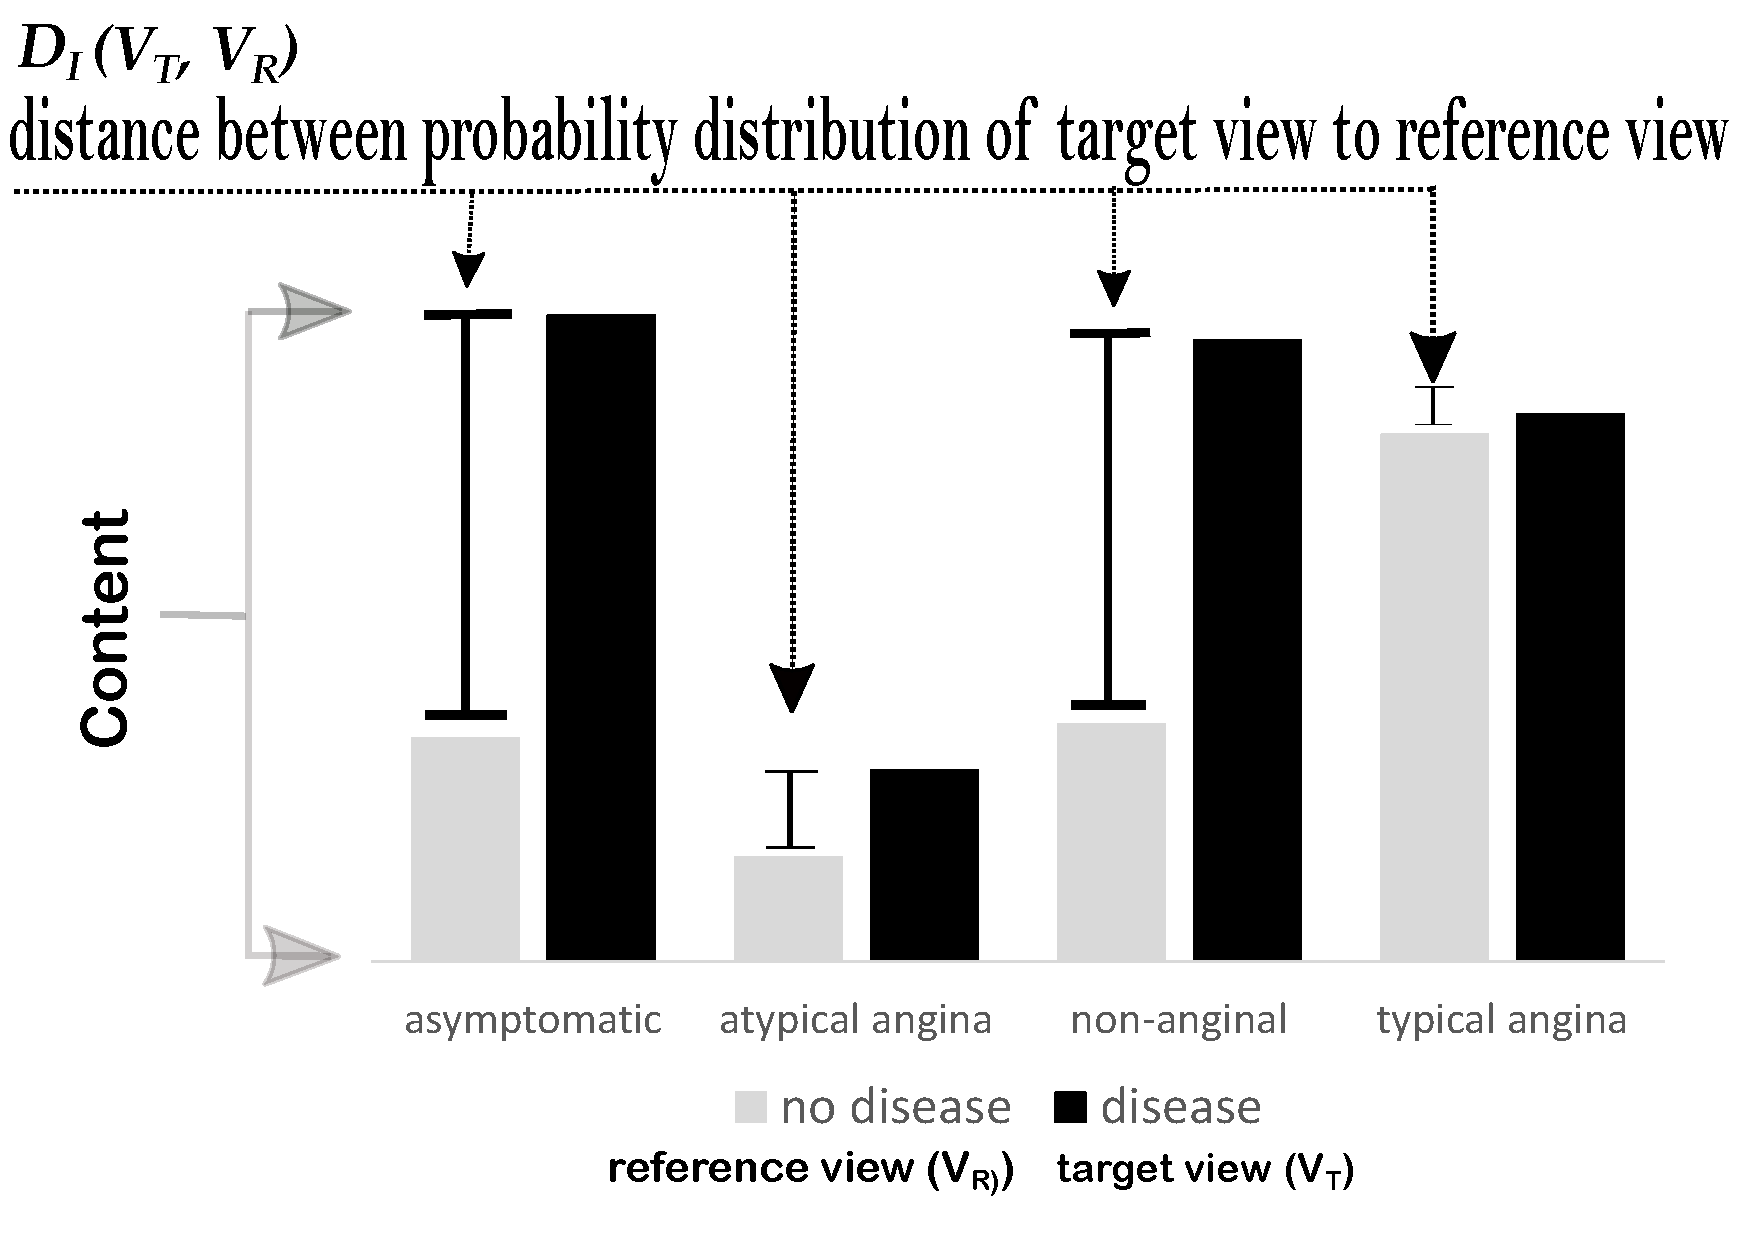
\includegraphics[width=2.5in]{figures/introduction/pre1}
		\caption{The content of view and the distance of $(V_T,V_R$)}
		\label{fig:pre1} 
	\end{subfigure}
	
	\begin{subfigure}[b]{0.40\textwidth}
		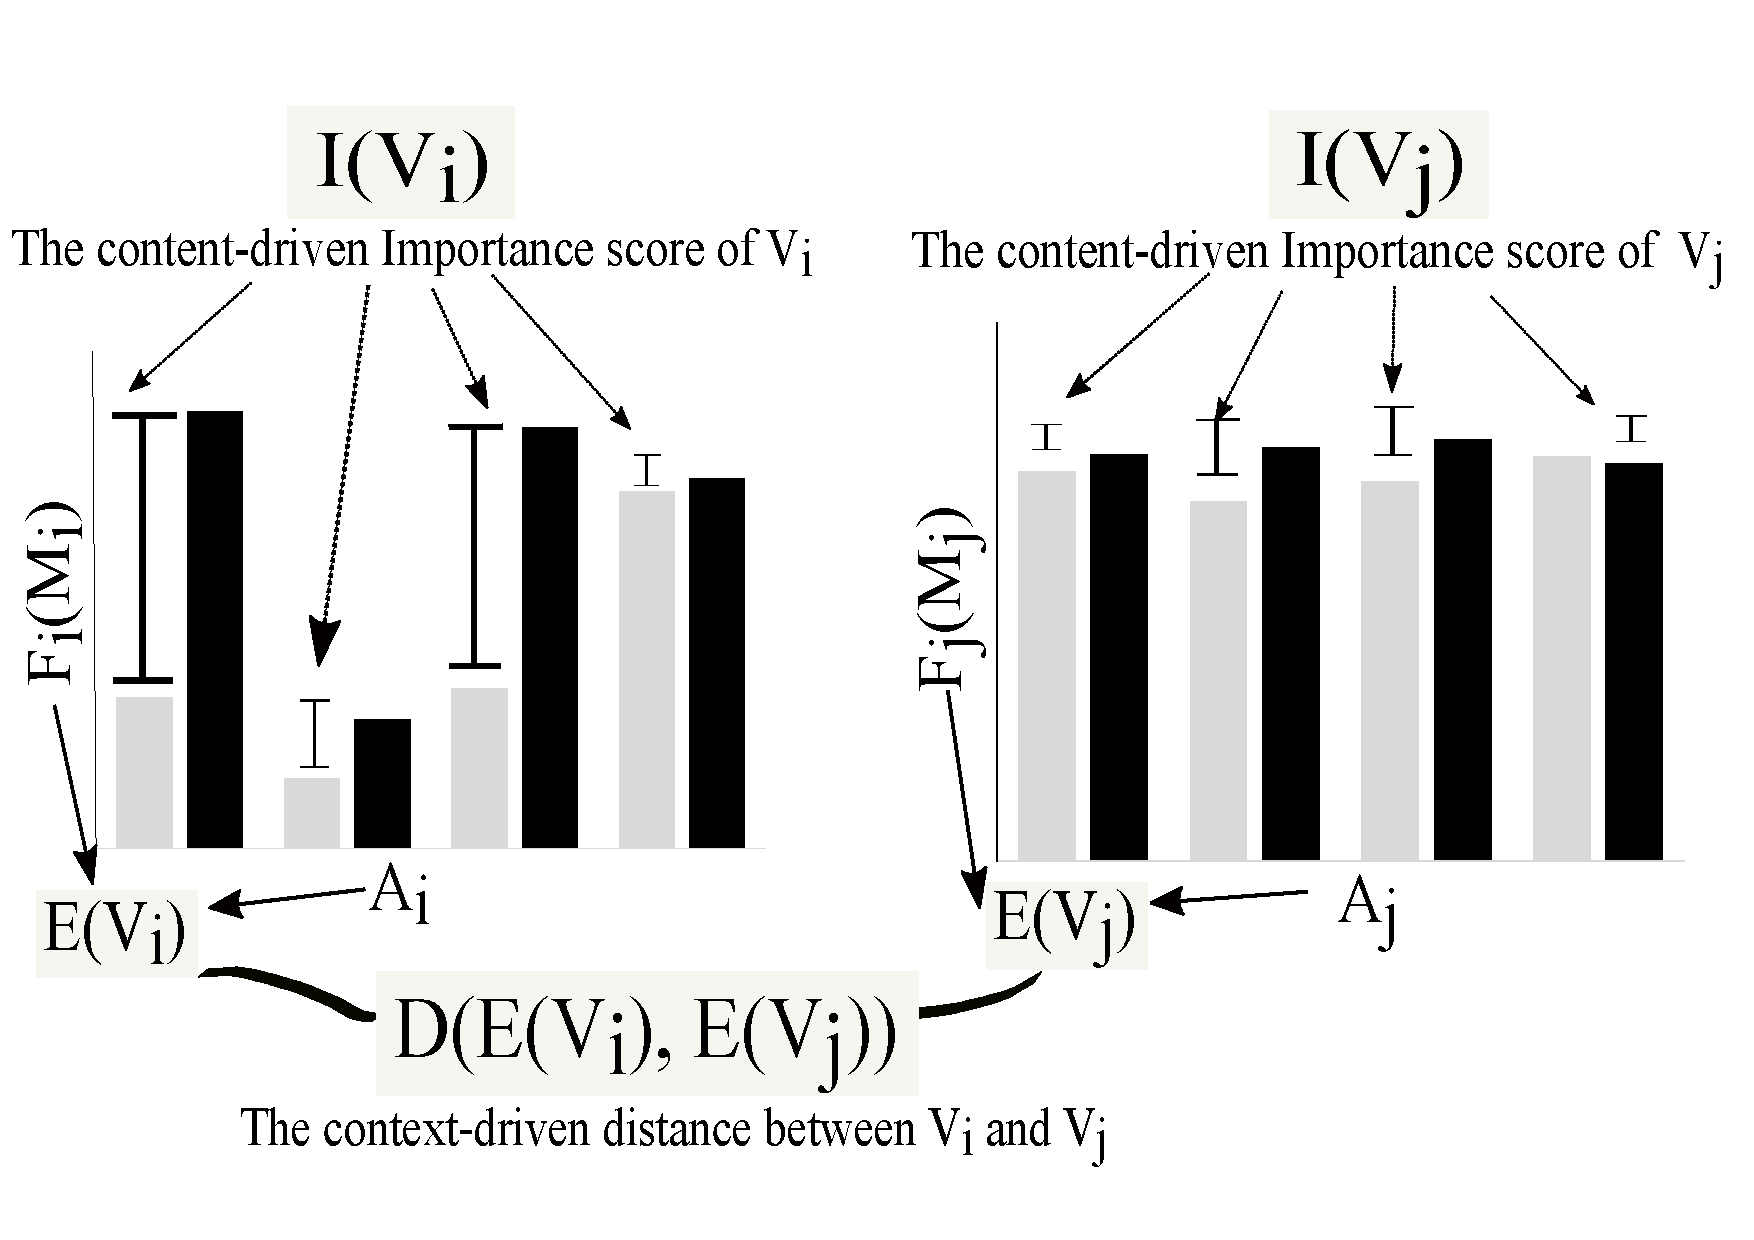
\includegraphics[width=2.5in]{figures/introduction/pre2}
		\caption{The context of views }
		\label{fig:pre2}
	\end{subfigure}
	\caption[content vs context]{Content vs. Context of views.}
	\label{fig:pre}
\end{figure}


The difference betweeen content and context is described in Figure \ref{fig:pre}. Content as in Figure \ref{fig:pre1} is the probability distribution of the aggregated query result whereas, Context as in Figure \ref{fig:pre2} is described as a set containing the name of the attribute, measure and function used to generate the view.  

\subsubsection{Content-Driven Deviation}
This approach measures how different a view is in relation to some reference subset of data. Hence, in order to compare the views, we need to have target subset and a reference subset of the $D_B$. The reference data set can either be another subset of $D_B$ or whole $D_B$. The example that we used are target subset $D_T$ is the subset of patients who has heart disease and the reference subset $D_R$ is the opposite, it consists of all patients without heart disease. For the content evaluation, we use a deviation-based approach as employed in \cite{Vartak2015}, \cite{Vartak2014}. The deviation value between target view and reference view is called as importance score. 

The importance score of $V_{T}$ is measured in terms of a score that captures the distance between probability distribution of target view $V_{T}$ over $D_T$ and probability distribution of reference view $V_{R}$  over $D_R$, it can be seen in Figure \ref{fig:pre1} and can be formally defined as follow:

\begin{equation}
D_I\left(V_T,V_R\right) = dist\left(\mathcal{P}\left[V_T\left(D_T\right)\right], \mathcal{P}\left[V_R\left(D_R\right)\right]\right)
\label{importance_score}
\end{equation}

where $ D_I\left(V_T,V_R\right) $ is the importance score of $ V_T$ and \textit{dist} is the Euclidian distance or other distance functions. To confirm that both views have the same scale, each view is normalized. The normalized probability distribution can be calculated by $ \frac{ Ag_1 }{G},\frac{ Ag_2 }{G},\frac{ Ag_3 }{G},\frac{ Ag_4}{G}.....,\frac{ Ag_n }{G} $ where $ \frac{Ag_i }{G}  $is the aggregated value of $ F $ over $ M $ for the group-by $ A $, and  $ G= $ $\sum_{p=1}^{n}{Ag_n}$. 

The higher distance between target view $ V_T $ and reference view $ V_R $, translates in to higher importance score $ D_I $. When judging the importance score of a view, it is believed that a view with large deviation from a reference view is more likely to reveal trends and patterns that are of high interest to the user \cite{Vartak2015}, \cite{Vartak2014}. 

\subsubsection{Context-Driven Deviation}
Content-driven deviation exposes the quality of individual view compared to reference view that can be other subsets of data or the whole data set. However, since the views are recommended as a collection or set which consists of multiple views, the quality of the whole set is as important as the quality of individual views\cite{Vartak2017}. The exiting approaches which only based on the content-driven only exposes the quality of individual view which are suffer from redundancy. To overcome this issue, we consider context-driven deviation that measures how different are the individual view within the set of views that recommended to the user. We believe that a diverse set of views is likely to be more informative than a monotonous set of views that have high importance score but provide little-added information relative to each other. 

To recommend a set of views which diverse among all views needs a diversity function. The notion of diversity has been widely used in recommendation systems for maximizing information gain and minimizing redundancy\cite{Zhang2008,Rafiei2010, Yu2009, Vieira2011}. There are various definitions of diversity, but most of them can be classified in one of this categories: (i) content-based diversity, means selecting results based on dissimilarity to each other \cite{Vieira2011,Khan2014}; (ii) novelty-based diversity selects the results that contain new information compared to the previous results which have been presented to the user\cite{Clarke2008}; (iii) semantic-based diversity selecting results that based on categories or topics\cite{Rafiei2010}. Depending on the type of recommendation system, different measures of diversity are used. 

For recommending a diverse set of visualizations, we deploy a diversity measure based on the context of the views. Intuitively, views generated using a different set of attributes, measures and functions are likely to provide different information. In order to determine the contextual distance between two views, we need to define a measure for calculating the distance between its context of two views. For instance, let $ V_i $ and $ V_j $ be two views that are generated using some aggregated queries over $D_Q$, and $ (ctx) $ means the context of the view. Also, let $ V_{i}(ctx) $= <$ A_i $,$ M_i $,$ F_i $> and $ V_{j}(ctx)=<A_j,M_j,F_j $> where { $ A_i , A_j \in \mathbb{A}, M_i, M_j \in \mathbb{M}, F_i, F_j \in \mathbb{F} $}. As comparing $ V_{i}(ctx)$ and $ V_{j}(ctx) $ require set comparison, we use Jaccard similarity measure which is a well-established similarity measure for sets of categorical data.  The Jaccard method measures similarity between finite sets as intersection of sets over union of sets. Hence, the Jaccard similarity between two views can be measured as:
\newline

\centerline{$ J$($V_{i}(ctx), V_{j}(ctx) $)$ = \dfrac{| V_{i}(ctx) \cap V_{j}(ctx) |}{| V_{i}(ctx) \cup V_{j}(ctx) |} $}
\bigskip

The contextual distance $ div $  between two views can be defined as: 
\newline
\begin{equation}
div\left(V_{i}(ctx), V_{j}(ctx)\right) = 1- J\left(V_{i}(ctx), V_{j}(ctx)\right) 
\label{diversity_score}                 
\end{equation}

% Diversity weight 

\bigskip
All symbols in this paper are explained in the Table of Symbols and it can be seen in Table \ref{tab:tab-symbols}.

\begin{table}
	\caption{Table of Symbols}
	\label{tab:tab-symbols}
	\begin{tabular}{ccl}
		\toprule
		Symbol &Description\\
		\midrule
		k & size of k\\
		S & selected set of views which equal to k\\
		S* & optimum set of views \\
		V & set of all possible generated views\\
		X & set of all remaining views which not included in S\\
		$ A $ & attribute / member of set of attributes $ \mathbb{A} $\\
		$ M  $& meassure  / member of set of meassures $ \mathbb{M} $\\
		$ F $ & agg. func. / member of set of agg. funcs. $ \mathbb{F} $\\
		$ Q $ & a general format for query \\
		$ T_T $ & a query predicate of the target subset\\
		$ T_R $ & a query predicate of the reference subset\\
		$ D_B  $& a multi-dimensional database \\
		$ D_Q  $& an example subset of $ D_B  $\\
		$ D_T  $& a target subset of $ D_B  $\\
		$ D_R  $& a reference subset of $ D_B  $\\\
		$ V_T  $& a target view\\
		$ V_R  $& a reference view \\
		$ V_i  $& an example of one view \\
		$ D_I$($S$)  & importance score of selected set of views\\
		$ div $  & the contextual distance between two views\\
		$ f$($S$,$div$) & diversity score of selected set of views\\
		$ F$($S$)  &  objective function value of the set S \\
		$ U$($V_i$) &  the utility score of each candidate view \\
		$ maxD_I$ &  the maximum value of importance\\
		\bottomrule
	\end{tabular}
\end{table}

\subsection{Problem Definition}
There are two main evaluation variables that used in this work, which are \textit{effectiveness} and \textit{efficiency}. The proposed recommendation visualization systems should recommend set of views with the high importance score as well as diverse among views. Moreover, it should has high efficiency in terms of costs due to all computations are running on the fly. 

\subsubsection{Effectiveness}
In this section, we formally define the problem of the quality of recommended views. \textit{i-DiVE} scheme designed to recommend a set of k views that are high importance as well as diverse among themselves. In particular, given a query subset $D_T$ as the target subset and a reference subset $D_R$ , set of all possible views V, our objective is to select a set  S* $\subseteq V $ where |S*| = k, such that the importance score of the views in S* and their mutual diversity is maximized. To achieve this goal, there are two components that need to be considered, the importance score of a set of views S, and the diversity score of the set S. 

\textit{The importance score computation}. The importance score of the set S is calculated as the normalized average value of the importance measure of each view in S, it can be defined as:
\newline

\centerline{$ D_I\left(S\right)= || \dfrac{1}{k} \sum_{i=1}^{k} D_I(V_i, V_R) ||, V_i  \in S $}
\bigskip

To normalize the importance score of set S to range 0 - 1, it can be by dividing the average of importance score of the set S with the maximum importance score. The maximum importance score of each views is not as straight forward, it depends on the real data. However, since the data generated by view is normalized (equation \ref{importance_score}), the range of the probability distribution representing each view is between 0 and 1. The maximum distance between two values in two different probability distributions can only be at most 1. Since, the sum of all values in a probability distribution can be 1, there can only be at most two pairs of values across two distributions with mutual distance of 1. This results in Euclidian distance of $ \sqrt{(1^2+1^2 )}= \sqrt{2} $. As a result, the maximum importance score to be equal to $\sqrt{2}$. 

\textit{The diversity score computation}. There are several diferent diversity functions have been employed in the literature \cite{Vieira2011,Khan2014},\cite{Clarke2008}, among which previous research has mostly focused on measuring diversity based on either the average or the minimum of the pairwise distances between elements of set \cite{Wu2014}. We focus on the first of those variants (i.e., average), as it considers all the views in S. Given a distance matric $ div\left(V_i, V_j\right) $ as given in equation 2, the diversity of a set S can be measured by a diversity function $ f\left(S,div\right) $ that captures the dissimilarity between the views in S, defined as:
\newline

$ f\left(S,div\right)= \dfrac{1}{k\left(k-1\right)}  \sum_{i=1}^{k} \sum_{j>i}^{k} div\left(V_i,V_j\right) ,V_i,V_j  \in S $
\newline

In order to capture both importance and diversity in the set of recommended views, we define a hybrid objective function that considers both importance and diversity when generating set S. Specifically, for a subset S $\subseteq V$ an objective function is formulated as the linear weighted combination of the diversity function $ f\left(S,div\right) $ and importance score, $ D_I\left(S\right) $ which is defined as:
\newline
\begin{equation}
F\left(S\right) =  \left(1-\lambda\right).D_I\left(S\right) + \lambda.f\left(S,div\right)
\label{objectif_function}
\end{equation}
\newline
where $ 0 \leq \lambda \geq 1 $ is employed to control the contribution between importance and diversity in the hybrid objective function. The higher values of $  \lambda $ result in a set of more diverse views whereas lower values of $ \lambda $ generate a set of the most important views that might be similar to each other. 
Given the hybrid objective function, our goal is to find an optimum set of views  $ S^* $ that maximizes the objective function $ F\left(S\right) $: 

\begin{equation}
S^* = \underset{\underset{|S|=k} {S \subseteq V}} {\mathrm{argmax}} F\left(S\right) 
\label{argmaxF}
\end{equation}



\subsubsection{Efficiency}
In the section before, we explained in terms of quality of the results which is presenting views based on importance and diversity. This section defines the issue in terms of efficiency, as explained in the preliminaries section that in case of the modest data which has small number of dimensions, it can generate large number of views. Meanwhile, views which want to be presented to users only in small number (top-k views) and all computation will be done on the fly. We need the scheme that robust in terms of the quality of results and also the running time (costs), in particular for the case of interactive visualization recommendation systems. 

It has been mentioned a lot in the literatures \cite{Vartak2014, Vartak2015, Ehsan2016} that the main issue of the visualization recommendation systems is the query execution. To deal with the query costs, there are several approaches that proposed, such as query results caching\cite{Khan2014}, shared computation among views, combine target and reference query, combination of multiple aggregates, combination of multiple group by, and parallel query and execution, \cite{Vartak2015},\cite{Wu2014}. 

However, in this work, we propose \textit{i-DiVE} scheme that equipped by pruning ability which able to reduce the number of query executions, the detail is presented in the proposed methods section. 











% ============================================== %
% PROPOSED METHODS %
% ============================================== %


\section{PROPOSED METHODS}

In this section, we present our \textit{i-DiVE} scheme for evaluating top-k visualizations that are of high importance to the user as well as diverse among themselves. Computing a set of top-k visualizations that maximize an objective function is a combinatorial optimization problem. Therefore, \textit{i-DiVE} employs Greedy algorithms which are popular for solving such optimization problems. Greedy algorithms have been shown to be efficient and provide good approximations to the optimal solutions \cite{Yu2009}, \cite{Vieira2011}, \cite{Smyth2001}. Generally, a Greedy algorithm starts with an empty set S and iteratively selects a view to be added to S that maximizes the objective function score $F\left(S\right)$. In most works, this approach is called Greedy Construction Algorithm. The key ingredient of any Greedy algorithm for solving an optimization problem is the Objective function itself that needs to be maximized. 

Before presenting the details of how \textit{i-DiVE} evaluates the hybrid objective function using greedy algorithm, we first present two baseline objective functions for evaluating top-k visualizations.

\subsection{Baseline Algorithms}

Current visualization recommendation systems consider only importance when ranking a view for recommendation \cite{Vartak2014, Vartak2015, Ehsan2016}. Thus, the objective function value of a set of k views S, is computed as the sum of the importance score of each view in S. This approach does not consider how the diversity score of S is effected when a new view is added to S. 
As discussed in the introduction, the recommendations generated solely on the basis of importance score, suffer from the redundancy problem.  The extreme solution to overcome the redundancy in the top-k set S is to select views such that the diversity score of S is maximized. This leads to two extreme baseline solutions, one based only on the importance score of the views and second based on only diversity score of the views. 

\begin{algorithm}
	\SetAlgoLined
	\KwIn{Set of views V and result set size k }
	\KwOut{Result set $ S \geq V $, |S| = k}  
	$S \leftarrow \left[v_i, v_j\right] $ get  two most distant views\;
	$X \leftarrow  \left[V \backslash S\right]$\;
	$i \leftarrow len\left(S\right) $\;
	\While{i < k}{
		\If{Pruning = True}{
		$ enablePruning $\;
		}
		\For{$j$ in set $X$}{
			$ max_v \leftarrow argmax F\left(X\left[j\right],S\right) $\;
		}
		$ S.add\left(max_v\right) $\;
		$ X.remove\left(max_v\right)$\;
		$ i  \leftarrow  i + 1 $\;
	}
	return S
	\caption{\textit{i-DiVE} Greedy}\label{i-DiVE-Greedy}
\end{algorithm}



\subsection{\textit{i-DiVE-Greedy} Scheme}

In order to capture both importance and diversity in the recommended top-k views, \textit{i-DiVE} employs a greedy construction algorithm to iteratively select views that maximize the hybrid objective function $F\left(S\right)$ as presented in equation 3, and it is called as \textit{i-DiVE-Greedy} scheme. The tradeoff between the importance score of a view and its distance from the already selected views in S, is controlled using the weight parameter $\lambda$. The smaller values of $\lambda$ can be selected by the user for a top-k set that contains views with high importance score. Whereas, the higher values of $\lambda$ can be selected for more diverse set of views. 
The details of the \textit{i-DiVE-Greedy} scheme are given in Algorithm \ref{i-DiVE-Greedy}. In particular, \textit{i-DiVE-Greedy} initializes the set S with two most distant views. The distance between all the views is calculated using the distance function as given in equation 2. In each iteration, a new view is selected from remaining views X and added to S. Thus, \textit{i-DiVE-Greedy} assigns a utility score to each candidate view which is based on the hybrid objective function $F\left(S\right)$ as defined in equation \ref{objectif_function}. The utility score of each candidate view $V_i$ in X is computed as: 

\begin{equation}
U\left(V_i\right)= \left(1-\lambda\right).D_I\left(V_i, V_R\right) + \lambda.setDist\left(V_i, S\right)
\label{utility_each_candidate}
\end{equation}

Where $ setDist\left(V_i, S\right) = \dfrac{1}{|S|} \sum_{\underset{V_j \in S}{j=1}}^{|S|} div\left(V_i, V_j\right) $
\newline

Thus, the view with highest utility score in each iteration is selected and added to S.

%\textit{i-DiVE-Greedy scheme costs.} There are four types of costs that required to run \textit{i-DiVE} scheme, as follows:
%
%\begin{itemize}
%	\item Query cost $C_Q$: Cost that needed for the query execution, the cost of $C_Q$ depends on the query itself and the number of rows (tuples) of the dataset. This cost depends on CPU and I/O cost but it dominated by I/O costs. 
%	\item Deviation/importance cost $ C_I $: The deviation computation cost is relatively cheap due to this cost only compute the probability distribution of each view and calculate the distance between two probability distribution of views (target view and reference view). The deviation equation can be seen in equation 1. This cost only from CPU costs.
%	\item Diversity cost $C_D$: Cost which required not only the computation of dissimilarity between two context views but also for whole diversity computation. This cost also only from CPU costs. $C_D$ depends on the number of views and the diversity algorithm that used, e.g. Greedy construction is cheaper than Swap, the cheapest is Random Algorithm. 
%	\item Visualization cost $C_V$: Cost which needed for plotting visualization and it only depends on CPU cost. 
%\end{itemize}

The time complexity of Greedy Construction algorithm has two components. One is the query execution cost for generating all views and computing the importance score $C_Q + C_I$. Second is the diversity cost $C_D$ that computing set distance of each view from the views already in S . The query execution cost is dominated by the I/O cost of retrieving the query results. Whereas, the set distance cost is the CPU cost of calculating the Jaccard similarity measure. The set distance cost is of $ O$($kn$) where k is the size of subset of views S and $ n $ is the number of all possible views. The query execution cost is of $ O$($n$) as the content of each view is generated only once. Although, greedy algorithm is very efficient as the number of attributes $\mathbb{A}$, measures $\mathbb{M}$ and aggregate functions $\mathbb{F}$, increase the number of views that need to be generated increase exponentially. Therefore, in order to reduce the cost of evaluating top-k views \textit{i-DiVE-Greedy} employs effective optimization strategy as elaborated next. 


\subsection{\textit{i-DiVE-Greedy} Optimization}

In order to recommend a small subset of views, the utility score of all possible views need to be computed. Since, the utility score of each view is based on its deviation from the reference view, the content of the view must be generated by executing the view query. However, only few views are eventually recommended to the user and rest of the views are discarded. Clearly, this approach would hinder the performance of the visualization recommendation systems for high dimensional datasets. Thus, motivated by the need to reduce the number of views that need to be generated, \textit{i-DiVE-Greedy} employs a pruning based optimization technique. 

The proposed optimization technique is based on the observation that the utility score of each view is a weighted sum of two different measures; 1) the importance score of view from the reference view and 2) diversity score of a view from S. The diversity score of a view requires only CPU computations and is thus a faster operation. Whereas, computing the importance score of a view by comparing the target view to the reference view incurs high I/O cost and CPU cost. The high I/O cost is dominated by the query executions. The CPU cost dominated from the computation of Euclidian distance between two probability distributions. 

Therefore, under that observation, \textit{i-DiVE-Greedy} leverages the diversity score of a view to decide whether a view query should be executed or not. Specifically, the views that will not make it to the recommended subset eventually, are identified early on the basis of their set distance score and are pruned. The view query is executed only for the remaining views to compute complete utility score for those views. For example, assume that a user wants to get some views from visualization recommendation systems and she uses $\lambda$ = 0.7. The $\lambda$ value equal to 0.7 means that the diversity score contribution to the utility score will be 70 percent and the contribution of the importance score will be 30 percent, as it can be seen in equation \ref{objectif_function}. Thus, on the basis of the diversity score only, low quality views can be pruned early. The details of the pruning method are given below.

We applied Max-Min pruning method as presented in \cite{Khan2015}. First, \textit{i-DiVE-Greedy} selects two most distant views as the initialization. In each iteration, instead of computing a complete utility score for each view, only partial utility score is computed. The partial utility score has two components; 1) the actual diversity score of the view from S and 2) the estimated importance score of view from the reference view. The partial utility score is defined as:

\begin{equation}
U'\left(V_i\right)= \left(1-\lambda\right).D_{I-est}\left(V_i, V_R\right) + \lambda.setDist\left(V_i, S\right)
\label{partial_utility}
\end{equation}
\newline
where  $ D_{I-est}\left(V_i,V_R\right) $ is the estimated importance score of $ V_i $ from $ V_R $. Without generating the view query, it is only possible to estimate the minimum and maximum deviation of a view from reference view. The minimum distance between two probability distributions can be 0 so we estimate minimum importance score as 0. The maximum importance score as explained in the preliminaries section is equal to $ \sqrt{2} $. Let us denote the minimum possible importance score of a view by $ minD_I\left(V_T,V_R\right) $ and maximum importance score by $ maxD_I\left(V_T,V_R\right) $.

Using the $ minD_I\left(V_i,V_R\right) $ and $maxD_I\left(V_i,V_R\right) $ values in the equation \ref{partial_utility}, we can calculate minimum utility score $ minU'\left(V_i\right) $ and maximum utility score $ maxU'\left(V_i\right) $  for all candidate views. The views that have $ maxU'\left(V_i\right) $  score less than the $ minU'\left(V_i\right) $score of any other view are pruned. This Max-Min pruning approach called as \textit{i-DiVE-Greedy-Static-Pruning}. This approach generates same set of recommended views as generated by the \textit{i-DiVE-Greedy} without pruning. This is due to the fact that in each iteration \textit{i-DiVE-Greedy } selects the view with highest utility score to be added to S. If the maximum possible utility score of a view is less than the minimum possible utility value of another view in the candidate list, it cannot be the winner with the highest utility score.

This Max-Min pruning approach has been mentioned in \cite{Khan2015} and it has good performance in pruning. However, in that literature, the points has very diverse values. To the contrary, in this work, the context of view only has three dimentions. Hence, by using three dimentions and computing the diversity score to small set of view S, the partial utility value may not diverse as in the literature. We were in doubt if this pruning scheme was able to prune significanly in this work. 

% it will be a good idea to discuss the characteristic of jaccard similiarity measure here. When comparing two sets with three items in each, there can only be three possible distance values, 1/3, 2/3 and 3/3. So pruning only on the basis of contextual distance may not be feasible for smaller lamda values. Then you can discuss why this problem is expected to not happen in the swap algorithm. %
\begin{algorithm}
	\SetAlgoLined
	\KwIn{Set of views V and result set size k }
	\KwOut{Result set $ S \geq V $, |S| = k}  
	$S \leftarrow $ Result set of only importance or only diversity\;
	$X \leftarrow  \left[V \backslash S\right]$\;
	$F_{current} \leftarrow 0 $\;
	$  improve \leftarrow  True $\;
	\While{improve = True}{
		%		\If{Pruning = True}{
		%			$ enablePruning $\;
		%		}
		\For{$i$ in set $X$}{
			$ S' \leftarrow S $\;
			\For{$j$ in set $S$}{
				\If{ $ F\left(S'\right) < F\left(S \backslash S[j] \cup X[i]\right) $}{
					$ S'  \leftarrow S \backslash j \cup X[i] $  \;
				}
			}
			\If{ $ F\left(S'\right) > F\left(S\right) $}{
				$ S  \leftarrow S'$
			}
		}
		\eIf{ $ F\left(S\right) > F_{current} $}{
			$ F_{current}   \leftarrow F\left(S\right) $\;
			$  improve \leftarrow  True $\;
		}{
		$  improve \leftarrow  False $\;
	}
}
return S
\caption{\textit{i-DiVE} Swap}\label{i-DiVE-Swap}
\end{algorithm}

\subsection{\textit{i-DiVE} Scheme using Swap technique}

Beside of using Greedy technique, we also proposed another approach which is using swap technique. Swap is local search type algorithm, this algorithm starts with a complete initial set S, and try to achieve better result by interchanging the remaining views in X to the current set S. If the views in remaining X able to give better objective function value $ F $($ S $), then this view will be joined to the current set and one view in the current set that has the lowest contribution to the $ F $($ S $) will be removed. 

In this work, we proposed two types of Swaps which are \textit{i-DiVE-SwapI} which is Swap algorithm that initialized by the results of Only Importance and \textit{i-DiVE-SwapD} which is Swap that initialized by results of Only Diversity. Both of those Swap algorithms already have a good initialization, \textit{i-DiVE-SwapI} with all current views in set S which has the maximum of importance score and \textit{i-DiVE-SwapD} with the current set S which has the maximum of diversity score. The details of \textit{i-DiVE-Swap} algorithm can be seen in Algorithm \ref{i-DiVE-Swap}.

The complexity of Swap algorithm is dependent on the query execution time, the importance score computation $ D_I\left(V_i,V_R\right) $ for all views, the diversity score and computation of objective function F(S) in each iteration. The importance score $ D_I\left(V_i,V_R\right) $ is calculated only once and is independent of the number of iterations of Swap. However, the objective function evaluation time is of $ O\left(k^2 \right) $ and the number of times objective function value is computed depends on the number of iterations of the swap and the number of views $ n $ in the candidate list. In the worst case, swap algorithm can perform $ O\left(k^n \right)  $iterations.



To minimize the I/O cost of executing view queries, we again apply pruning method in Swap algorithm. \textit{i-DiVE-SwapI} uses the results of Only importance as the first initialization. Hence, in case of reducing query executions by pruning scheme, this algorithm cannot escape from executing all queries due to this algorithm uses result set of Only importance in the initialization that required to execute all queries in advanced. However, the second proposed swap algorithm which is \textit{ i-DiVE-SwapD}, this algorithm uses the result of Only Diversity as the set of initialization. This algorithm does not need importance score for the initialization, it means there is no query execution for the initialization and pruning scheme can be applied on it. The detail of \textit{ i-DiVE-SwapD} optimization using pruning scheme is explained below. 

\begin{algorithm}
	%	\SetAlgoLined
	%	\KwIn{Set of views V and result set size k }
	%	\KwOut{Result set $ S \geq V $, |S| = k}  
	%	$S \leftarrow $ Result set of only importance or only diversity\;
	%	$X \leftarrow  \left[V \backslash S\right]$\;
	%	$F_{current} \leftarrow 0 $\;
	%	$  improve \leftarrow  True $\;
	$ max_b  \leftarrow\sqrt{2} $\;
	%$ X' \leftarrow [] $\;
	\For{$i$ in set $X$}{
		\For{$j$ in set $S$}{
			$ d  \leftarrow setDist\left(X[i],S \backslash S[j]\right) $\;
			$ 	newX \leftarrow [S[j], X[i], d]$\;
			$ 	X'.append(newX)$\;
		}
	}
	$ 	X' \leftarrow sorted\_by\_d(X') $\;
	$ S' \leftarrow S $\;
	\eIf{ $ max_b == \sqrt{2} $}{
		\For{$i$ in set $X'$}{
			
			\If{ $ F\left(S'\right) < F\left(S \backslash X'[i][0] \cup X'[i][1], max_b\right) $}{
				$ 	X''.append(X'[i][1])$\;
			}
		}
		
		$n \leftarrow pi - len(S)$\;
		$samples \leftarrow X''[0\colon n]$\;
		$maxI\_S \leftarrow get\_maxI(S)$\;
		$maxI\_samples \leftarrow get\_maxI(samples)$\;
		
		\If{ $ maxI\_S > maxI $}{
			$ maxI \leftarrow maxI\_S$
		}
		\If{ $ maxI\_samples> maxI $}{
			$ maxI \leftarrow maxI\_samples$
		}
		$max\_b \leftarrow maxI$	
		
		\For{$i$ in set $X''$}{
			\For{$j$ in set $S$}{
				\If{ $ F\left(S'\right) < F\left(S \backslash S[j] \cup X''[i], max_b\right)  $}{
					$ 	X'''.append(X''[i])$\;
					$ I \leftarrow get\_I\_score(X''[i]) $\;
					\If{ $ F\left(S'\right) < F\left(S \backslash S[j] \cup X''[i], I\right) $}{
						$ S'  \leftarrow S \backslash j \cup X''[i] $  \;
					}
					\If{ $ I > max_b $}{
						$ max_b \leftarrow I $
					}
				}
			}
		}
		
	}{ 
	\For{$i$ in set $X'$}{$ .... $
		%			\If{ $ F\left(S'\right) < F\left(S \backslash X'[i][0] \cup X'[i][1]\right) $}{
		%				$ 	X''.append(X'[i][1])$\;
		%			}
		%			$ I \leftarrow get\_I\_(X''[i]) $\;
		%			\If{ $ F\left(S'\right) < F\left(S \backslash S[j] \cup X''[i], max\_bound\right) $}{
		%				$ S'  \leftarrow S \backslash j \cup X''[i] $  \;
		%			}
		%			\If{ $ I > max\_bound $}{
		%				$ max\_bound \leftarrow I $
		%			}
		
	}
	
}

\If{ $ F\left(S'\right) > F\left(S\right) $}{
	$ S  \leftarrow S'$
}
return S
\caption{\textit{i-DiVE} SwapD Pruning}\label{i-DiVE-SwapD-Pruning}
\end{algorithm}

\subsection{\textit{i-DiVE-SwapD} Optimization}

In order to apply pruning scheme in \textit{i-DiVE-SwapD}, as in the Greedy technique, we utilize the maximum importance score $maxD_I$. To run \textit{i-DiVE-SwapD}, for the first time, $maxD_I$ will be initialized by $\sqrt{2}$. All views in X will be tried one by one to the current set S. In each iteration, instead of computing a complete utility score for each view, only partial utility score is computed, as in equation \ref{partial_utility}. The partial utility score using actual value of diversity score and estimated value of importance score $maxD_I$ which is equal to $\sqrt{2}$.

If the view in X, by using importance score $maxD_I$ which is equal to $\sqrt{2}$ cannot perform better in terms of improving the objective function value to the current set S, those views will be pruned. This method is valid due to if the importance score set to the maximum and that view cannot improve the objective function of the current set, then there is no reason to know the actual value of importance by executing the query of that view. The pruning scheme which applied in \textit{i-DiVE-SwapD} is called \textit{i-DiVE-SwapD-Static-Pruning}.


% Compare with Greedy in terms of pruning performance%

\subsection{Adaptive Pruning Scheme}

All proposed pruning schemes including \textit{i-DiVE-Greedy-Static-Pruning} and \textit{i-DiVE-SwapD-Static-Pruning} are using static value of $maxD_I$ which is equal to $\sqrt{2}$. The main issue of using static value of $maxD_I$ is if the estimated value of maximum importance score $maxD_I$ too far from the real value of the importance score in the dataset, the pruning scheme may not working optimal. 

In order to get better performance of pruning scheme, instead of using static $maxD_I = \sqrt{2} $, we proposed Adaptive Pruning scheme, that can adapt the value of $maxD_I$ to the real values in the dataset. In order to estimate the $maxD_I$ which can close to the real value in the dataset, we use sampling method. 

We applied this adaptive pruning scheme to \textit{i-DiVE-Greedy} algorithm which called \textit{i-DiVE-Greedy-Adaptive-Pruning} and to \textit{i-DiVE-SwapD} algorithm as called \textit{i-DiVE-SwapD-Adaptive-Pruning} . 

%For instance, in the \textit{i-DiVE-SwapD-Adaptive-Pruning}, $maxD_I$ is initialized by $ \sqrt{2} $. If the view by using $maxD_I$ can improve the objective function value in the current set S, the real Importance score of this view will be computed which is by executing the query of its view. For instance, after executing its query, the real Importance value is 0.25, by using $ \alpha= 0.8 $, the $ EWMA_t  $ will be $ (0.8 *0.25) + ((1- 0.4)*\sqrt{2}) = 0.48 $, and the current $maxD_I$ will be set to 0.48, and it will be updated continuously. This EWMA method able to set the value of $maxD_I$ as close as the real values in the dataset, it should make pruning scheme works better. 











% ============================================== %
% EXPERIMENTAL EVALUATION %
% ============================================== %


\section{EXPERIMENTAL EVALUATION}

\begin{table}
	\caption{Parameters testbed in the experiments}
	\label{tab:tab-parameter}
	\begin{tabular}{ccl}
		\toprule
		Parameter &Range (\textbf{default})\\
		\midrule\
		datasets & Flights, \textbf{Heart disease}, Superstore\\
		sample queries & \textbf{10} \\
		diversity weight ratio & \textbf{3($ A $) : 2($ M $) : 1($ F $)} \\
		tradeoff weight $ \lambda $ & 0, 0.2, 0.4, \textbf{0.5}, 0.6, 0.8, 1 \\
		result set (size of \textit{k}) & \textbf{5}, 15, 25, 35\\
		prediction interval (PI) \% & 80 , 85, 90, 95, \textbf{97}, 98\\
		\bottomrule
	\end{tabular}
\end{table}

\begin{table*}
	\centering
	\caption{The list of Schemes (Algorithms)}
	\label{tab:tab-list-schemes}
	\begin{tabular}{ccl}
		\toprule
		Scheme &Description\\
		\midrule\
		
		Only Importance & Consider only importance \\
		Only Diversity   & Consider only diversity\\
		i-DiVE-Greedy & Consider both importance and diversity (Hybrid) using Greedy technique\\
		i-DiVE-SwapI & Hybrid using Swap technique and the initialization set generated by Only Importance \\
		i-DiVE-SwapD & Hybrid using Swap technique and the initialization set generated by Only Diversity \\
		i-DiVE-Greedy-Static-Pruning & i-DiVE-Greedy equipped with pruning scheme which use static max bound = $ \sqrt{2} $\\
		i-DiVE-Greedy-Adaptive-Pruning & i-DiVE-Greedy equipped with pruning scheme that uses adaptive max bound\\
		i-DiVE-SwapD-Static-Pruning &i-DiVE-SwapD equipped with pruning scheme that uses static max bound = $ \sqrt{2} $ \\
		i-DiVE-SwapD-Adaptive-Pruning & i-DiVE-SwapD equipped with pruning scheme that uses adaptive max bound\\
		\bottomrule
	\end{tabular}
\end{table*}

% Experiment Setup and Dataset % 

\textbf{\textit{Experiment Setup}}. This experiment running on Windows 10 64 bit, Intel Core i7-7700 CPU @ 3.60 GHz, RAM 16 GB. The experiment is developed using Python and run on Python version 3.6.3 with PostgreSQL as the database engine. In this experiments, we use three real datasets, as follows: 

\begin{itemize}
	\item Airline Dataset \footnote{http://stat-computing.org/dataexpo/2009/the-data.html}, it has 7 attributes, 4 measure attributes. The detail as follows: $ \mathbb{A}  $= year, month, week, day, carrier, origin, destination; $ \mathbb{M}  $= arrivaldelay, departurdelay, weatherdelay, distance. This dataset has 855,632 number of rows. 
	\item Heart Disease Dataset \footnote{http://archive.ics.uci.edu/ml/datasets/heart+Disease}, it has 14 attributes in total which are 9 attributes $ \mathbb{A} $ and 5 measure attributes $ \mathbb{M} $, $ \mathbb{A}  $= sex, cp, fbs, restecg, exang, slope, ca, thal, num; $ \mathbb{M} $ = age, trestbps, chol, thalach, oldpeak. This dataset has small number of rows (299 rows).
	\item Tableau Superstore Dataset \footnote{https://community.tableau.com/docs/DOC-1236}, it has 13 attributes, 4 measure attributes. The detail as follows: $ \mathbb{A} $= order\_date, ship\_date, ship\_mode, customer\_name, segment, country, state, region, city, postal\_code, category, subcategory, product\_name; $ \mathbb{M} $ = sales, quantity, discount, profit. There are 10,971 rows of this dataset.
\end{itemize}

% i-DIVE schemes compared to BF and Random % 

%\textbf{\textit{i-DiVE schemes performance compared to Brute Force and Random}}. Before we start to analyze the effectiveness and the efficiency of our proposed schemes, to check its performance, we run all schemes and compared to all baselines including Brute Force and Random selection. We run all schemes only using k=5 due to BF algorithm has running time limitation, BF complexity is $O$($n^k k^2$). Hence, it is not good idea to increase the number of k due to BF algorithm tests every possibility of the result set, it should has the highest overall objective function value $F\left(S\right)$ among all proposed schemes. Moreover, all algorithms also should have better performance than the Random algorithm. The results show that two extreme baselines (Only Importance and Only Diversity) are not able to acheive the optimal overall objective function value $F\left(S\right)$. Only importance that only considers importance score, the value of $D_I$($S$) almost same as BF algorithm but $f$($S,div$) worse than Random. To the contrary, Only Diversity that only consider diversity value, it has high $f$($S,div$) which very closes to the BF algorithm but $D_I$($S$) close to Random. 
%Other than that, our proposed schemes either based on Greedy technique or Swap have overall objective function value $F\left(S\right)$ close to BF and better than those two extreme baselines. 



%\begin{figure*}[t]
%	\centering
%	\subcaptionbox{Flight dataset}[.3\linewidth][c]{%
%		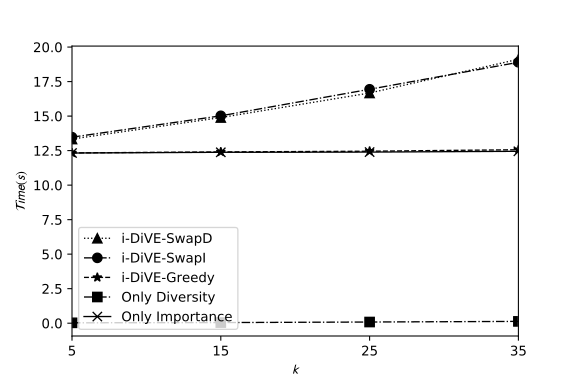
\includegraphics[width=.33\linewidth]{figures/results/output_time_flights}}\quad
%	\subcaptionbox{Heart disease dataset}[.3\linewidth][c]{%
%		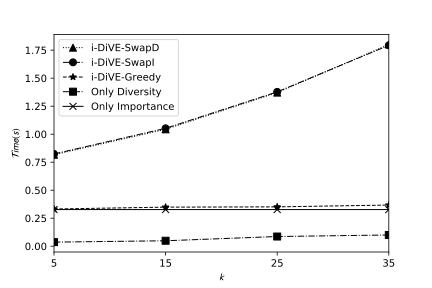
\includegraphics[width=.33\linewidth]{figures/results/output_time_heart}}\quad
%	\subcaptionbox{Superstore dataset}[.3\linewidth][c]{%
%		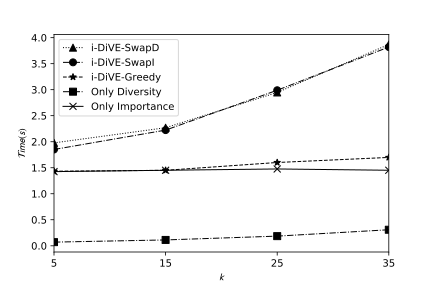
\includegraphics[width=.33\linewidth]{figures/results/output_time_superstore}}
%	\caption{Overall Costs/execution time while running on real datasets}	
%\end{figure*}

\begin{figure*}[t]
	\centering
	\subcaptionbox{Flights dataset}[.3\linewidth][c]{%
		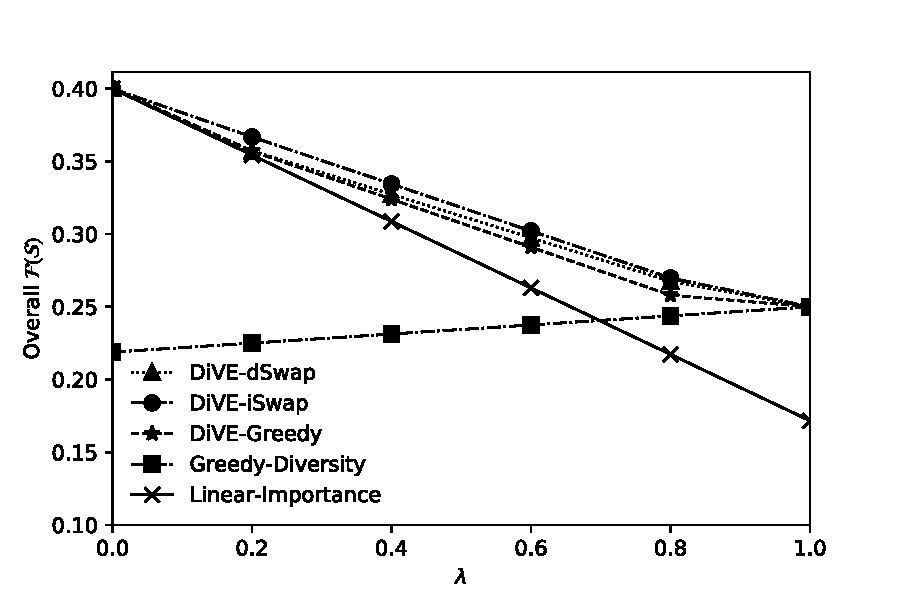
\includegraphics[width=.33\linewidth]{figures/results/tradeoff_flights}}\quad
	\subcaptionbox{Heart disease dataset}[.3\linewidth][c]{%
		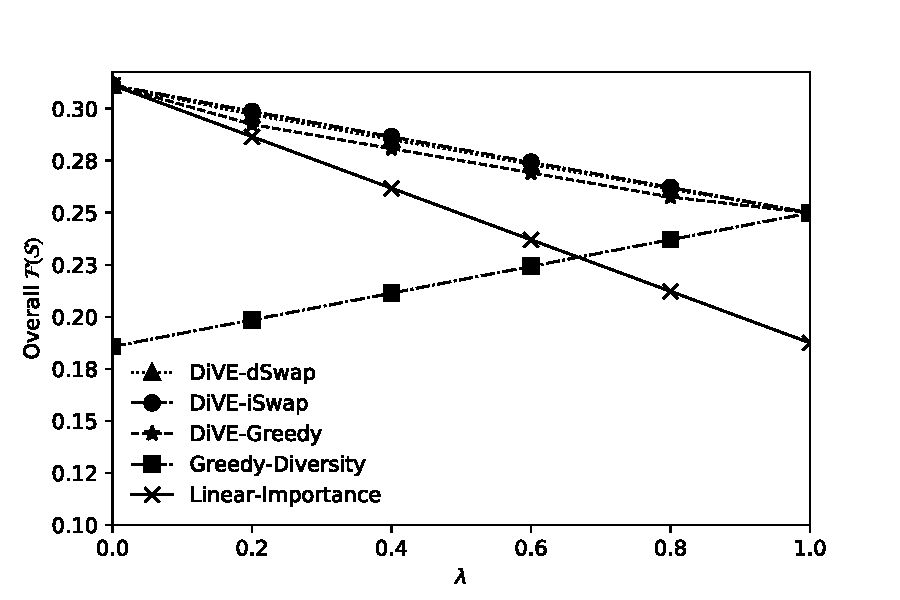
\includegraphics[width=.33\linewidth]{figures/results/tradeoff_heart_2}}\quad
	\subcaptionbox{Superstore dataset}[.3\linewidth][c]{%
		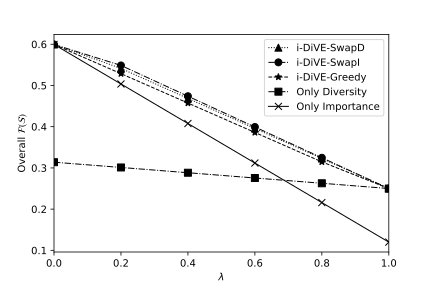
\includegraphics[width=.33\linewidth]{figures/results/tradeoff_superstore}}
	\caption{Impact of $\lambda$ to overall objective function value $F\left(S\right)$ while k = 5 and running on three real datasets}
	\label{fig:tradeoff_3_datasets}	
\end{figure*}

\begin{figure*}[t]
	\centering
	\subcaptionbox{Flights datasets}[.3\linewidth][c]{%
		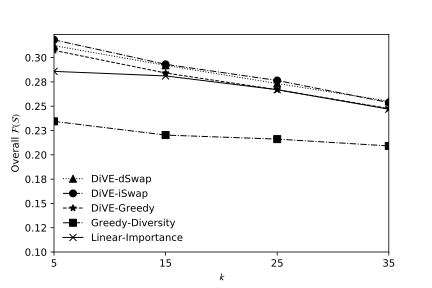
\includegraphics[width=.33\linewidth]{figures/results/objf_flights}}\quad
	\subcaptionbox{Heart disease dataset}[.3\linewidth][c]{%
		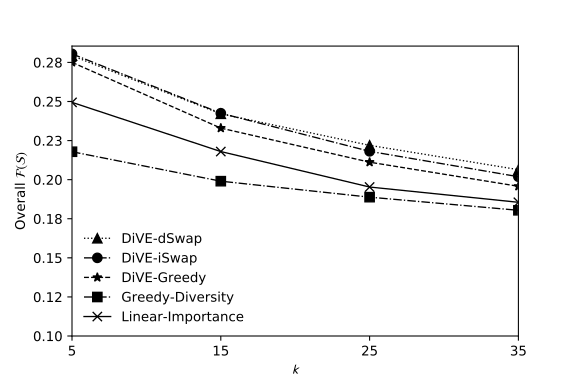
\includegraphics[width=.33\linewidth]{figures/results/objf_heart_2}}\quad
	\subcaptionbox{Superstore dataset}[.3\linewidth][c]{%
		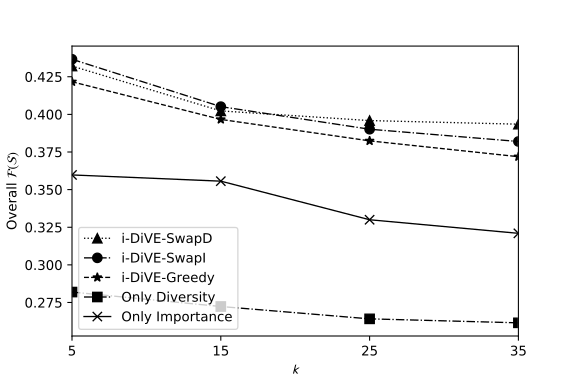
\includegraphics[width=.33\linewidth]{figures/results/objf_superstore}}
	\caption{Overall objective function value $F\left(S\right)$ using different value of k and running on three real datasets}
	\label{fig:objf_3_datasets}
\end{figure*}


\subsection{Effectiveness Evaluation}
%  Prolog of the quality of the results evaluation%
To test the performance of our proposed approach, we run the experiments using three real datasets which are flights dataset, heart disease dataset, and superstore dataset. In order to present the representative result, for each dataset, we execute ten random queries as shown in Table \ref{tab:tab-parameter}. Afterwards, we calculate the average of all results as the final result. We examine the performance of our proposed schemes in term of the quality of the result (effectiveness) and the efficiency. The detail results of the experiments which using different value of parameters as summarized in Table \ref{tab:tab-parameter} is elaborated next. 
 
 % The Impact of \lambda to the overall objective function value %
 
\textbf{\textit{The impact of parameter weight $\lambda$ to the overall $F\left(S\right)$}}. One of the advantage \textit{i-DiVE} scheme is users can decide what kind of the results that they want by changing the value of weight $\lambda$. The main function of $\lambda$ is this weight can be used to tradeoff between importance and diversity, it is explained in equation \ref{objectif_function}. Figure \ref{fig:tradeoff_3_datasets} shows the impact of $\lambda$ to the overall objective values $F\left(S\right)$ by fixed k equal to 5, where $ 0 \leq \lambda \geq 1 $. We can see in this figure that in the beginning when the $\lambda$ is close to 0, means the role is dominated by the importance score, Only importance has high overall objective function value $F\left(S\right)$ but it will decline gradually while increasing of $\lambda$. To the contrary, the Only Diversity is the opposite, it has the high overall objective function value when the $\lambda$ equal to 1, which means the diversity gets the full role. Hence, there is a crossover between Only importance and Only Diversity, this crossover shows the role balancing between importance score and diversity score. Futhermore, our proposed schemes have stable performance in all various $\lambda$ value and its  $F\left(S\right)$ value always better than Only importance and Only diversity. 

\begin{figure}
	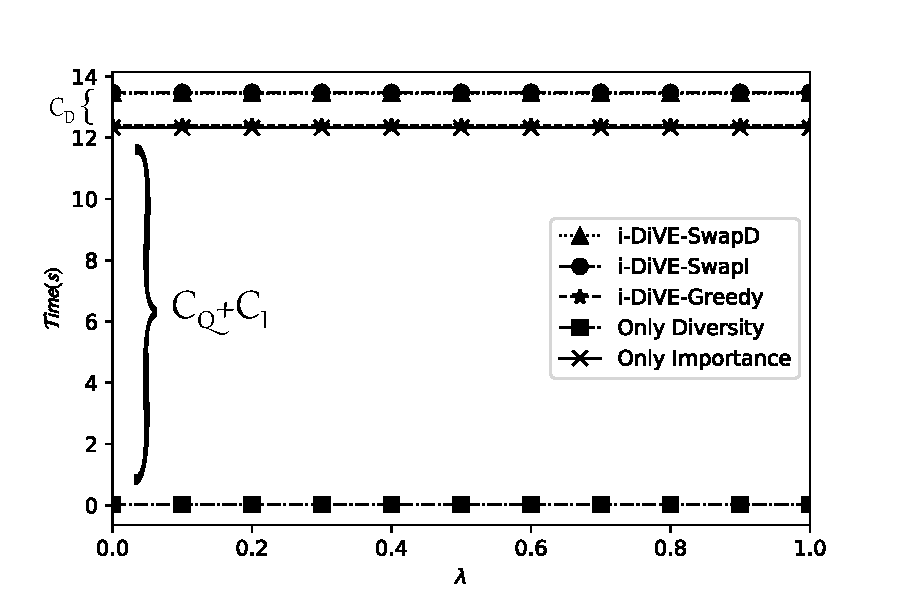
\includegraphics[width=3in]{figures/results/output_time_flights_lambda}
	\caption{Total time in seconds to execute schemes on flights dataset using k =5. It shows that costs are dominated by query costs}
	\label{fig:cost_flights}
\end{figure}

In addition, as shown in Figure \ref{fig:tradeoff_3_datasets}, there is unbalance between importance score of the set $D_I$($S$) and diversity score of set $f$($S,div $). It can be seen by the shape of the graphs while increasing the value of $\lambda$. When $\lambda$ value is small, the overall objective function value in the highest position and it decrease gradually while $\lambda$ is increased.  It happens due to unbalance of the real value of importance score and diversity score. The range value of diversity score can be predicted. As mentioned in the preliminaries section, this work uses three combination of context of the view which is $A, M, F$ (attributes, measures, and aggregate functions). According to the equation \ref{diversity_score}, the range value of diversity score is between 0 and 1. Let assume that the number of k equal to 3, to calculate the dissimilarity among three views that each view has three dimensions, the diversity value of the set which contains of three views $f$($S,div $) will be less than 0.5. As we know that the diversity value of set $f$($S,div $) decrease while k is increasing. On the other hand, the importance score cannot be predicted, the real value of importance depends on the real value inside the dataset. We only know that the maximum of importance score is $\sqrt{2}$. Due to this reason, it is not surpising if the shape of the graphs are not balance. The real importance score of the set $D_I$($S$) can be seen while the $\lambda$ = 0, in this moment, there is no contribution for diversity. Otherwise, the real diversity score of the set $f$($S,div $) can be seen while the $\lambda$ = 1.0. 




 % The Impact of k to the overall objective function value %
 
\textbf{\textit{The impact of k to the overall objective function value $F\left(S\right)$}}. It has been explained the impact of $\lambda$ to the overall objective function value $F\left(S\right)$. In this section, we explain the overall objective function value $F\left(S\right)$ by increasing k. Figure \ref{fig:objf_3_datasets} shows the overall objective values $F\left(S\right)$ by using different number of k. As shown in those figures, the value of $F\left(S\right)$ decrease while increasing the value of k. There are two reasons why this moment happens. First, to get the importance score from the set $D_I$($S$), sum of all importance score of views will be divided by the number of views or the number of k, increasing the number of k means increasing the divisor. Second, the diversity score of a set of views $f$($S,div $) also depends on the number of k. While k is increasing, the diversity score of the set will decrease, due to the score of $f$($S,div $) is yielded from the sum of all distance of views divided by $ k*(k-1)$. Hence, the more views selected, the probability to get similar views will be high and the score of diversity will be declined. 

The most important point in this results is our proposed schemes always have better overall objective function value $F\left(S\right)$ compared to the two extreme baselines in various number of k. Overall, the rank of the scheme performance in terms of the overall objective function value $F\left(S\right)$, start from the highest are \textit{i-DiVE-SwapI}, \textit{i-DiVE-SwapD}, and \textit{i-DiVE-Greedy} respectively.   



\subsection{Efficiency and Pruning Scheme Evaluation}

% Efficiency and Pruning Scheme%

\begin{figure}
	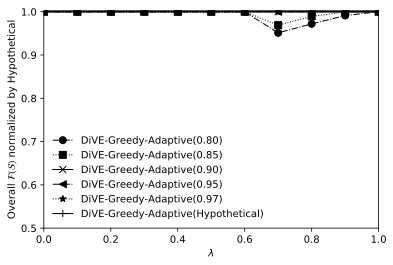
\includegraphics[width=2.9in]{figures/results/impact_lambda_to_PI_sampling_greedy_pruning}
	\caption{Impact of $ \lambda  $ to the performance of \textit{i-DiVE-Greedy-Adaptive-Pruning} with different of PI in terms of the effectiveness, running on Heart disease dataset using k = 5. Using PI 80 and PI 85 can reduce the quality of the result while the $\lambda$ value is low}
	\label{fig:impact_lambda_to_PI_sampling_greedy_pruning}
\end{figure}
\begin{figure}
	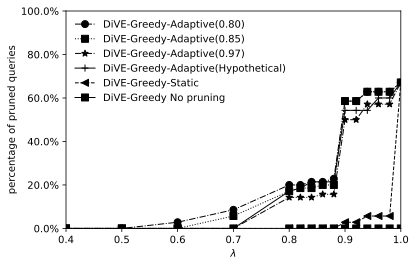
\includegraphics[width=2.9in]{figures/results/pruning_performance_greedy}
	\caption{Impact of $\lambda$ to the pruned queries of \textit{i-DiVE-Greedy} scheme, running on Heart disease dataset using k = 5. Using PI-97 able to prune queries around 20 percent while $\lambda$ higher than 0.8}
	\label{fig:pruning_performance_greedy}
\end{figure}


% Overall execution time / Overall costs to run all schemes%

\textbf{\textit{The total of execution time to run proposed schemes}}. In order to start analyzing the efficiency, we need to know the main issue in term of costs. Figure \ref{fig:cost_flights} shows the example of exactly time that needed to run schemes on flights dataset. It shows Only Diversity which only considering diversity and no query executions, it has very cheap in total costs. The costs of Only diversity almost same as Random even it closes to 0. Meanwhile, Only importance and \textit{i-DiVE-Greedy} seems in the same line but that was not exactly same. The total of diversity computations $ C_D $ of \textit{i-DiVE-Greedy} is very low, the total costs of \textit{i-DiVE-Greedy} is dominated by query costs $ C_Q $. Due to of this reason, the total execution time of \textit{i-DiVE-Greedy} closes to Only importance. Those are the proof that the total costs of all schemes execpt Only diversity are dominated by query cost $ C_Q $. 

The highest cost is the query cost $ C_Q $ in all datasets. However, heart disease dataset is the exception due to this dataset only has 299 rows, it is a very small dataset, due to this reason, the diversity cost $ C_D $ of Swap algorithms on k equal to 5 is higher than the query cost $ C_Q $, it only happens when the dataset is very small. 

\begin{figure}
	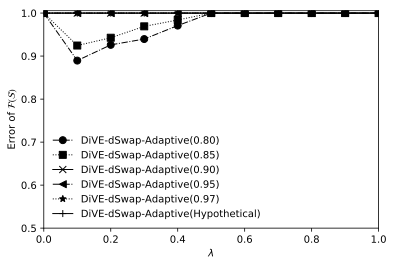
\includegraphics[width=2.9in]{figures/results/impact_lambda_to_PI_sampling_swapd_pruning}
	\caption{Impact of $ \lambda  $ to the performance of \textit{i-DiVE-SwapD-Adaptive-Pruning} with different of PI in terms of the effectiveness, running on Heart disease dataset using k = 5. Using PI 80 and PI 85 can reduce the quality of the result while the $\lambda$ value is low}
	\label{fig:impact_lambda_to_PI_sampling_swapd_pruning}
\end{figure}
\begin{figure}
	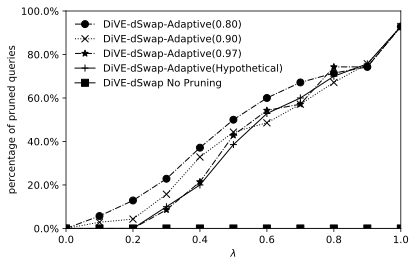
\includegraphics[width=2.9in]{figures/results/pruning_performance_swapd}
	\caption{Impact of $\lambda$ to the pruned queries of \textit{i-DiVE-SwapD} scheme, running on Heart disease dataset using k = 5. Adaptive pruning schame able to prune queries start from $\lambda$ 0.1, it has more pruned queries while $\lambda$ increased}
	\label{fig:pruning_performance_swapd}
\end{figure}


Due to the page limitation, all our experiments in three real dataset cannot be showed. Hence, for the next sections, we use heart disease dataset as our focus observation. 
% Static Pruning Scheme Performance%

%\subsubsection{Static-Pruning scheme performance}


% Impact of lambda (parameter to tradeoff between importance and diversity) to the pruned queries, running on Heart disease dataset %

\textbf{\textit{Impact of $\lambda$ to the pruned queries of \textit{i-DiVE-Greedy} scheme}}. In this work, we proposed two kind of pruning schemes, that are using estimated static value of maximum value of the importance score $maxD_I$ and using adaptive maximum value of importance score. 

The first our pruning scheme is using static value $maxD_I$. To check the performance of our pruning scheme, we run it to all real datasets using different value of $ \lambda $. We analyze the result by comparing the result of schemes with pruning enable on it and the schemes without pruning enable on it. The example result which running on heart disease dataset is shown in Figure \ref{fig:pruning_performance_greedy} . The static pruning scheme only able to prune queries while the value of $\lambda$ is high, closes to 0.9. As we expected, it is because the value of $maxD_I$ that too far from the real value of importance score. 

%\subsubsection{Adaptive-Pruning scheme performance}
To overcome the flaw in static pruning scheme, we also proposed adaptive pruning scheme which used dynamic value of the maximum importance score $maxD_I$. In order to get $maxD_I$ as close as possible to the real value of importance in the dataset, we applied sampling method. By using adaptive pruning, users also able to change the confidence and the margine error to tradeoff between time and precision. 

% Impact of lambda to the pruned queries for adaptive pruning scheme %

\textbf{\textit{Impact of $\lambda$ to the pruned queries of \textit{i-DiVE-SwapD} scheme}}. If static pruning scheme only able to prune queries while $\lambda$ closes to 0.9 and higher, in this section, we shows the adaptive pruning performance. Figure \ref{fig:pruning_performance_swapd} shows the performance of adaptive pruning scheme by using different value of $\lambda$. It shows the impact of $\lambda$ to the percentage of pruned queries. The adaptive pruning schemes especially \textit{i-DiVE-SwapD-Adaptive-Pruning} is able to prune queries significantly, pruning start while $\lambda$ closes to 0.2 and by increasing the $\lambda$, more queries can be pruned.


% The impact of query load to the pruning performance %

\textbf{\textit{The impact of query load to the pruning performance}}. As shown in Figure \ref{fig:objf_3_datasets}, that the actual value of importance score affects to the overall value of objective function $F\left(S\right)$ and the shape of the graphs. The next question is do the actual value of importance score also affects the pruning performance while using adaptive pruning scheme? We did experiments using heart disease dataset to answer this question. We lists all subsets in the heart disease dataset and classify those subsets to three categories: low, middle, and high. Low category consist of subsets that have mostly low value of importance score, high category is the opposite, and the middle category is the middle of low and high. We compare the result in terms of pruning performance using input low, middle, and high categories. The result can be seen in Figure \ref{fig:low_vs_high}. It has different result while using low category and high category. Input using low category or low query load has more pruned queries compared to high query load (high category).

In addition, most of subsets in the heart disease dataset are in the middle category, this finding explains the Figure 4b, the shape of heart disease graph is more balanced compare to flights and superstore dataset. If mostly subsets in heart disease dataset are middle category the probability 10 selection of random queries in the middle category is high.  










% The impact of Random sorted method to the pruning performance %



% ============================================== %
% RELATED WORK  %
% ============================================== %


%\section{RELATED WORK}
%
%There are a lot of visualization tools which commonly used by users but most current visualization tools that exist today do not support auto-generated recommended views. As we know, Tableau starts to provide the feature \quotes{Show Me}\cite{Tableau}, that provides recommended chart type of visualization. Tableau used VizQL \cite{Hanrahan2006} which the previous version called \cite{Stolte2002} Polaris to automatically generates recommended chart types. It happens when the user starts to select the attribute of the dataset, Tableau \quotes{Show Me}\cite{Tableau} provides recommended charts that match the selected attributes. However, this feature only recommends chart types not recommend the subset which has interesting trends.  The recent work that developed visualization recommendation systems is SeeDB \cite{Vartak2015}, \cite{Vartak2014}, the authors using a statistical method to compute the probability distribution of each subset of the dataset. They compare the probability distribution of the selected subset to another subset or whole dataset. The subset which has a high deviation/distance matrics from reference subset (another subset/whole dataset) can be defined as interesting views. 
%
%%Another recent work of visualization recommendation systems is Voyager \cite{Wongsuphasawat2016} which based on Vega-lite \cite{Satyanarayan2017}. Voyager uses statistical properties of the data to generate recommended views while Vega-lite is new high-level specification language, it using JSON object to describe the data source, it also called a new grammar of interactive graphic.
%
%To understand user interests and giving the recommended items that can satisfy the users in recommendation system is a non-trivial task. There have been many studies in developing algorithms that boost prediction accuracy of recommended items in recommendation system but it was not enough. In some case, high accuracy produces homogenous recommended items and high accuracy does not guarantee users satisfactory. Some researchers proposed the importance of diversification, they argued that diverse items mean more opportunities for users to get the satisfied items \cite{Adomavicius2012}. Diversification also has been known as the NP-hard problem \cite{Erkut1990}. 
%%Moreover, several works which proposing diversification in recommendation system can be seen in \cite{Zhang2008}, and  \cite{Yu2009}. In addition, this comprehensive survey \cite{Zheng2017} explained details about the definition of diversification, its classification, also including techniques and algorithms, and real implementation of diversification such as in database system, recommendation system, search engines and soon. 
%Several techniques have been proposed for diversification, the best known algorithm for this technique is greedy solution\cite{Yu2009}, \cite{Vieira2011}, \cite{Smyth2001}. This work \cite{Gollapudi2009} proposed several natural axioms which showed that there is no diversification objective that can satisfy all the axioms simultaneously. Another work \cite{Vieira2011} presented an experimental evaluation of various common query result diversification techniques such as greedy, swap, random, motley, clustering, etc.




% ============================================== %
% CONCLUSIONS %
% ============================================== %

\section{Conclusions}
In this paper, we proposed \textit{i-DiVE} scheme which the main purposes are to evaluates and optimizes the results of visualization recommendation systems with respect to importance and diversity. The advantage of \textit{i-DiVE} is that users can set their preferences by changing the parameter to tradeoff between importance and diversity to get result set. We also performed an experimental study and present the results which focus on effectiveness and efficiency of our approach on real datasets. We proposed \textit{i-DiVE} scheme which based on Greedy and Swap approach, \textit{i-DiVE-SwapI} have the best performance in recommending result views but it has the highest costs due to this scheme executing all possible view from the dataset, this scheme can be used for the user who only cares about the results without worrying execution time. However, to the users who care about execution time, we proposed \textit{i-DiVE-SwapD-Adaptive-Pruning} and \textit{i-DiVE-Greedy-Adaptive-Pruning}, those schemes can decrease costs significantly without reducing the quality of results.
%\end{document}  % This is where a 'short' article might terminate



\begin{figure}
	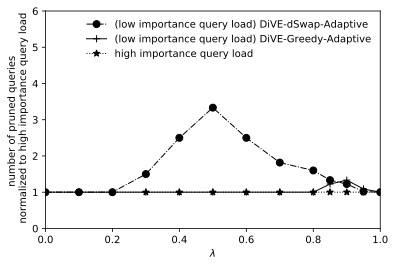
\includegraphics[ width=2.8in]{figures/results/low_vs_high}
	\caption{Number of pruned queries of high and low query load normalized by high query load using different value of $\lambda$, k = 5 and running on Heart disease dataset}
	\label{fig:low_vs_high}
\end{figure}

%
%\appendix
%%Appendix A
%\section{Headings in Appendices}
%The rules about hierarchical headings discussed above for
%the body of the article are different in the appendices.
%In the \textbf{appendix} environment, the command
%\textbf{section} is used to
%indicate the start of each Appendix, with alphabetic order
%designation (i.e., the first is A, the second B, etc.) and
%a title (if you include one).  So, if you need
%hierarchical structure
%\textit{within} an Appendix, start with \textbf{subsection} as the
%highest level. Here is an outline of the body of this
%document in Appendix-appropriate form:
%\subsection{Introduction}
%\subsection{The Body of the Paper}
%\subsubsection{Type Changes and  Special Characters}
%\subsubsection{Math Equations}
%\paragraph{Inline (In-text) Equations}
%\paragraph{Display Equations}
%\subsubsection{Citations}
%\subsubsection{Tables}
%\subsubsection{Figures}
%\subsubsection{Theorem-like Constructs}
%\subsubsection*{A Caveat for the \TeX\ Expert}
%\subsection{Conclusions}
%\subsection{References}
%Generated by bibtex from your \texttt{.bib} file.  Run latex,
%then bibtex, then latex twice (to resolve references)
%to create the \texttt{.bbl} file.  Insert that \texttt{.bbl}
%file into the \texttt{.tex} source file and comment out
%the command \texttt{{\char'134}thebibliography}.
% This next section command marks the start of
% Appendix B, and does not continue the present hierarchy
%\section{More Help for the Hardy}
%
%Of course, reading the source code is always useful.  The file
%\path{acmart.pdf} contains both the user guide and the commented
%code.

\begin{acks}
	This research is supported by the Indonesia Endowment Fund for Education (LPDP) as scholarship provider from the Ministry of Finance, Republic of Indonesia.
	Big thanks to Dr. Hina A Khan who help to fixing the gramatical error and giving the inputs to this work. 
	
\end{acks}
